% Author: Cyrille Chenavier, Christophe Cordero, Samuele Giraudo
% Creation: may. 2018
% Modifications: may. 2018, june 2018, july 2018

\documentclass[10pt,reqno]{amsart}

%%%%%%%%%%%%%%%%%%%%%%%%%%%%%%%%%%%%%%%%%%%%%%%%%%%%%%%%%%%%%%%%%%%%%%%%
%%%%%%%%%%%%%%%%%%%%%%%%%%%%%%%%%%%%%%%%%%%%%%%%%%%%%%%%%%%%%%%%%%%%%%%%
%%%%%%%%%%%%%%%%%%%%%%%%%%%%%%%%%%%%%%%%%%%%%%%%%%%%%%%%%%%%%%%%%%%%%%%%
\usepackage[utf8x]{inputenc}
\usepackage[english]{babel}
\usepackage{amsmath,amsfonts,amssymb,amsthm,shuffle}
\usepackage[T1]{fontenc}
\usepackage[math]{anttor}

% Layout.
\usepackage[top=3.5cm,bottom=3.5cm,left=3.6cm,right=3.6cm]{geometry}

% Colors of hyperlinks.
\usepackage{xcolor}
% Author: Samuele Giraudo
% Creation: mar. 2018
% Modifications: mar. 2018

\definecolor{ColBlack}{RGB}{0,0,0} % Black.
\definecolor{ColWhite}{RGB}{255,255,255} % White.
\definecolor{Col1}{RGB}{133,6,6} % Rouge sang.
\definecolor{Col2}{RGB}{198,8,0} % Rouge ponceau.
\definecolor{Col3}{RGB}{174,74,52} % Rouge tomette.
\definecolor{Col4}{RGB}{103,113,121} % Gris de Payne.
\definecolor{Col5}{RGB}{90,94,107} % Ardoise.
\definecolor{Col6}{RGB}{70,63,50} % Taupe.

\newcommand{\ColBlack}[1]{\textcolor{ColBlack}{#1}}
\newcommand{\ColWhite}[1]{\textcolor{ColWhite}{#1}}
\newcommand{\ColA}[1]{\textcolor{Col1}{#1}}
\newcommand{\ColB}[1]{\textcolor{Col2}{#1}}
\newcommand{\ColC}[1]{\textcolor{Col3}{#1}}
\newcommand{\ColD}[1]{\textcolor{Col4}{#1}}
\newcommand{\ColE}[1]{\textcolor{Col5}{#1}}
\newcommand{\ColF}[1]{\textcolor{Col6}{#1}}


\usepackage[hyperindex=true,frenchlinks=true,colorlinks=true,
citecolor=Col2,linkcolor=Col3,urlcolor=Col4,linktocpage,
pagebackref=true]{hyperref}

% Tikz.
\usepackage{tikz}
\usetikzlibrary{shapes}
\usetikzlibrary{fit}
\usetikzlibrary{decorations.pathmorphing}
\usetikzlibrary{arrows.meta}

% Misc.
\usepackage{mathtools}
\usepackage{dsfont}
\usepackage{wasysym}
\usepackage{stmaryrd}
\usepackage{cite}
\usepackage{subfig}
\usepackage{multirow}
\usepackage{enumitem}
\usepackage{multicol}
\usepackage{cancel}

%%%%%%%%%%%%%%%%%%%%%%%%%%%%%%%%%%%%%%%%%%%%%%%%%%%%%%%%%%%%%%%%%%%%%%%%
%%%%%%%%%%%%%%%%%%%%%%%%%%%%%%%%%%%%%%%%%%%%%%%%%%%%%%%%%%%%%%%%%%%%%%%%
%%%%%%%%%%%%%%%%%%%%%%%%%%%%%%%%%%%%%%%%%%%%%%%%%%%%%%%%%%%%%%%%%%%%%%%%
% Line space.
\linespread{1.15}
\renewcommand{\arraystretch}{1.4}

% Vertical space for equations.
\setlength{\abovedisplayskip}{5pt}
\setlength{\belowdisplayskip}{5pt}

% Alphabetic footnote marks.
\renewcommand{\thefootnote}{\alph{footnote}}

% To allow cutting equations in several pages.
\allowdisplaybreaks

% Numbering of equations.
\numberwithin{equation}{subsection}

% Depth of the table of contents.
\setcounter{tocdepth}{2}

% Indentation in the table of contents.
\makeatletter
\def\l@section{\@tocline{1}{3pt}{1pc}{5pc}{}}
\def\l@subsection{\@tocline{2}{2pt}{2pc}{5pc}{}}
\makeatother

% Environments definitions.
\newtheorem{Theorem}{Theorem}[subsection]
\newtheorem{Proposition}[Theorem]{Proposition}
\newtheorem{Lemma}[Theorem]{Lemma}

% Better comparison symbols.
\renewcommand{\leq}{\leqslant}
\renewcommand{\geq}{\geqslant}

% Mathematical symbols

%%%%%%%%%%%%%%%%%%%%%%%%%%%%%%%%%%%%%%%%%%%%%%%%%%%%%%%%%%%%%%%%%%%%%%%%
%%%%%%%%%%%%%%%%%%%%%%%%%%%%%%%%%%%%%%%%%%%%%%%%%%%%%%%%%%%%%%%%%%%%%%%%
%%%%%%%%%%%%%%%%%%%%%%%%%%%%%%%%%%%%%%%%%%%%%%%%%%%%%%%%%%%%%%%%%%%%%%%%
\title{Comb associative operads}
\keywords{Operad; trees; Rewrite rule; Presentation; Enumeration.}
\subjclass[2010]{\Todo{}}
\date{\today}
\author{Cyrille Chenavier \and Christophe Cordero \and Samuele Giraudo}
\address{\scriptsize Université Paris-Est, LIGM (UMR $8049$), CNRS,
    ENPC, ESIEE Paris, UPEM, F-$77454$, Marne-la-Vallée, France}
\email{cyrille.chenavier@u-pem.fr}
\email{christophe.cordero@u-pem.fr}
\email{samuele.giraudo@u-pem.fr}

%%%%%%%%%%%%%%%%%%%%%%%%%%%%%%%%%%%%%%%%%%%%%%%%%%%%%%%%%%%%%%%%%%%%%%%%
%%%%%%%%%%%%%%%%%%%%%%%%%%%%%%%%%%%%%%%%%%%%%%%%%%%%%%%%%%%%%%%%%%%%%%%%
%%%%%%%%%%%%%%%%%%%%%%%%%%%%%%%%%%%%%%%%%%%%%%%%%%%%%%%%%%%%%%%%%%%%%%%%
% Author: Samuele Giraudo
% Creation: mar. 2018
% Modifications: mar. 2018

% Tools macros.
\newcommand{\Todo}[1]{\textcolor{Col1}{{\tt TODO: $[$#1$]$}}}
\newcommand{\Hide}[1]{\textcolor{Col4}{\tt [hidden]}}

% Format macros.
\newcommand{\Def}[1]{\textcolor{Col3}{\em #1}}
\newcommand{\OEIS}[1]{\href{http://oeis.org/#1}{{\bf #1}}}
\newcommand{\Arxiv}[1]{\href{https://arxiv.org/abs/#1}{\tt arXiv:#1}}

% Tikz for vertical centering.
\tikzstyle{Centering}=[{baseline={([yshift=-0.5ex]current
    bounding box.center)}}]


\newcommand{\N}{\mathbb{N}}
\newcommand{\Z}{\mathbb{Z}}
\newcommand{\Q}{\mathbb{Q}}
\newcommand{\K}{\mathbb{K}}

\newcommand{\Oca}{\mathcal{O}}
\newcommand{\Rfr}{\mathfrak{r}}
\newcommand{\Sfr}{\mathfrak{s}}
\newcommand{\Tfr}{\mathfrak{t}}

\newcommand{\Zero}{\mathtt{0}}
\newcommand{\Two}{\mathtt{2}}
\newcommand{\HilbertSeries}{\mathcal{H}}
\newcommand{\GeneratingSet}{\mathfrak{G}}
\newcommand{\FreeOperad}{\mathrm{F}}
\newcommand{\Mag}{\mathbf{Mag}}
\newcommand{\QMag}{\mathcal{Q}\left(\Mag\right)}
\newcommand{\IMag}{\mathcal{I}\left(\Mag\right)}
\newcommand{\As}{\mathsf{As}}
\newcommand{\CAs}[1]{\mathsf{CAs}^{(#1)}}
\newcommand{\CAsAll}{\mathbf{CAs}}
\newcommand{\PrefixWord}{\mathrm{p}}
\newcommand{\Deg}{\mathrm{deg}}
\newcommand{\LComb}[1]{\mathfrak{c}^{(#1)}_{\diagup}}
\newcommand{\RComb}[1]{\mathfrak{c}^{(#1)}_{\diagdown}}
\newcommand{\LRank}{\mathrm{lr}}
\newcommand{\RBranch}{\mathrm{rb}}
\newcommand{\Catalan}{\mathrm{cat}}
\newcommand{\OrdCAs}{\preceq}
\newcommand{\Unit}{\mathds{1}}
\newcommand{\Leaf}{\perp}
\newcommand{\Corolla}{\mathrm{c}}
\newcommand{\NormalForms}{\mathfrak{N}}

\DeclareMathOperator{\Product}{\star}
\DeclareMathOperator{\Congr}{\equiv}
\DeclareMathOperator{\Rew}{\to}
\DeclareMathOperator{\RewRT}{\overset{*}{\Rew}}
\DeclareMathOperator{\RewT}{\overset{+}{\Rew}}
\DeclareMathOperator{\RewRTS}{\overset{*}{\leftrightarrow}}
\DeclareMathOperator{\RewContext}{\Rightarrow}
\DeclareMathOperator{\RewContextT}{\overset{+}{\RewContext}}
\DeclareMathOperator{\RewContextRT}{\overset{\ast}{\RewContext}}
\DeclareMathOperator{\RewContextRST}{\overset{\ast}{\Leftrightarrow}}
\DeclareMathOperator{\lcm}{lcm}

\newcommand{\CongrCAs}[1]{\Congr^{(#1)}}

% Tree drawings.
\tikzstyle{Node}=[circle,draw=Col1!80,fill=Col1!8,inner sep=1pt,
minimum size=2mm,thick,font=\scriptsize]
\tikzstyle{Edge}=[draw=Col2!80,cap=round,thick]
\tikzstyle{EdgeColorF}=[Edge,draw=Col6!90,ultra thick]
\tikzstyle{Leaf}=[rectangle,draw=ColBlack!70,fill=ColBlack!16,
inner sep=0pt,minimum size=1mm,thick]
\tikzstyle{NodeST}=[font=\footnotesize]
\tikzstyle{Injection}=[ColBlack!100,draw,
{>[scale=1.5,length=4,width=5]}-{>[scale=1.5,length=4,width=5]}]
\tikzstyle{Map}=[ColBlack!100,draw,-{>[scale=1.5,length=4,width=5]}]

%%%%%%%%%%%%%%%%%%%%%%%%%%%%%%%%%%%%%%%%%%%%%%%%%%%%%%%%%%%%%%%%%%%%%%%%
%%%%%%%%%%%%%%%%%%%%%%%%%%%%%%%%%%%%%%%%%%%%%%%%%%%%%%%%%%%%%%%%%%%%%%%%
%%%%%%%%%%%%%%%%%%%%%%%%%%%%%%%%%%%%%%%%%%%%%%%%%%%%%%%%%%%%%%%%%%%%%%%%
\begin{document}

%%%%%%%%%%%%%%%%%%%%%%%%%%%%%%%%%%%%%%%%%%%%%%%%%%%%%%%%%%%%%%%%%%%%%%%%
%%%%%%%%%%%%%%%%%%%%%%%%%%%%%%%%%%%%%%%%%%%%%%%%%%%%%%%%%%%%%%%%%%%%%%%%
%%%%%%%%%%%%%%%%%%%%%%%%%%%%%%%%%%%%%%%%%%%%%%%%%%%%%%%%%%%%%%%%%%%%%%%%
\begin{abstract}
    The associative operad is the quotient of the magmatic operad by
    the operad congruence identifying the two binary trees of degree
    $2$. We introduce here a generalization of the associative operad
    depending on a nonnegative integer $d$, called $d$-comb associative
    operad, as the quotient of the magmatic operad by the operad
    congruence identifying the left and the right comb binary trees of
    degree $d$. We study the case $d = 3$ and provide an orientation
    of its space of relations by using rewrite systems on trees and
    the Buchberger algorithm for operads to obtain a convergent
    rewrite system.
\end{abstract}

\maketitle

\tableofcontents

%%%%%%%%%%%%%%%%%%%%%%%%%%%%%%%%%%%%%%%%%%%%%%%%%%%%%%%%%%%%%%%%%%%%%%%%
%%%%%%%%%%%%%%%%%%%%%%%%%%%%%%%%%%%%%%%%%%%%%%%%%%%%%%%%%%%%%%%%%%%%%%%%
%%%%%%%%%%%%%%%%%%%%%%%%%%%%%%%%%%%%%%%%%%%%%%%%%%%%%%%%%%%%%%%%%%%%%%%%
%%%%%%%%%%%%%%%%%%%%%%%%%%%%%%%%%%%%%%%%%%%%%%%%%%%%%%%%%%%%%%%%%%%%%%%%
%%%%%%%%%%%%%%%%%%%%%%%%%%%%%%%%%%%%%%%%%%%%%%%%%%%%%%%%%%%%%%%%%%%%%%%%
%%%%%%%%%%%%%%%%%%%%%%%%%%%%%%%%%%%%%%%%%%%%%%%%%%%%%%%%%%%%%%%%%%%%%%%%
\section*{Introduction}
Associative algebras are spaces endowed with a binary product $\Product$
satisfying among others the associativity law
\begin{equation}
    \left(x_1 \Product x_2\right) \Product x_3
    =
    x_1 \Product \left(x_2 \Product x_3\right).
\end{equation}
It is well-known that the associative algebras are representations of
the associative (nonsymmetric) operad $\As$. This operad can be seen as
the quotient of the magmatic operad $\Mag$ (the free operad of binary
trees on the binary generator~$\Product$) by the operad
congruence~$\Congr$ satisfying
\begin{equation} \label{equ:congruence_as}
    \begin{tikzpicture}[xscale=.24,yscale=.24,Centering]
        \node(0)at(0.00,-3.33){};
        \node(2)at(2.00,-3.33){};
        \node(4)at(4.00,-1.67){};
        \node[NodeST](1)at(1.00,-1.67)
            {\begin{math}\Product\end{math}};
        \node[NodeST](3)at(3.00,0.00)
            {\begin{math}\Product\end{math}};
        \draw[Edge](0)--(1);
        \draw[Edge](1)--(3);
        \draw[Edge](2)--(1);
        \draw[Edge](4)--(3);
        \node(r)at(3.00,1.5){};
        \draw[Edge](r)--(3);
    \end{tikzpicture}
    \Congr
    \begin{tikzpicture}[xscale=.24,yscale=.24,Centering]
        \node(0)at(0.00,-1.67){};
        \node(2)at(2.00,-3.33){};
        \node(4)at(4.00,-3.33){};
        \node[NodeST](1)at(1.00,0.00)
                {\begin{math}\Product\end{math}};
        \node[NodeST](3)at(3.00,-1.67)
                {\begin{math}\Product\end{math}};
        \draw[Edge](0)--(1);
        \draw[Edge](2)--(3);
        \draw[Edge](3)--(1);
        \draw[Edge](4)--(3);
        \node(r)at(1.00,1.5){};
        \draw[Edge](r)--(1);
    \end{tikzpicture}\,.
\end{equation}
These two binary trees are the syntax trees of the expressions appearing
in the above associativity law.
\medbreak

In a more combinatorial context and regardless of the theory of operads,
the Tamari order is a partial order on the set of the binary trees
having a fixed number of internal nodes $\gamma$. This order is
generated by the covering relation consisting in rewriting a tree $\Tfr$
into a tree $\Tfr'$ by replacing a subtree of $\Tfr$ of the form of the
left member of~\eqref{equ:congruence_as} into a tree of the form of the
right member of~\eqref{equ:congruence_as}. This transformation is known
in a computer science context as the right rotation
operation~\cite{Knu98} and intervenes in algorithms involving binary
search trees~\cite{AVL62}. The partial order hence generated by the
right rotation operation is known as the Tamari order~\cite{Tam62} and
has a lot of combinatorial and algebraic properties (see for
instance~\cite{HT72,Cha06}).
\medbreak

A first connection between the associative operad and the Tamari order
is based upon the fact that the orientation of~\eqref{equ:congruence_as}
from left to right provides a convergent orientation (a terminating and
confluent rewrite relation) of the congruence $\Congr$. The normal
forms of the rewrite relation induced by the rewrite rule obtained by
orienting~\eqref{equ:congruence_as} from left to right are right comb
binary trees and are hence in one-to-one correspondence with the
elements of~$\As$. Following the ideas developed by Anick for
associative algebras~\cite{Ani86}, the description of an operad by mean
of normal forms provides homological information for this operad. One of
the fundamental homological properties for operads is
Koszulness~\cite{GK94}, generalizing Koszul associative
algebras~\cite{Pri70}: the convergent orientation of $\As$ proves that
it is a Koszul operad~\cite{LV12}.
\medbreak

This work is intended to study and collect the possible links between
the Tamari order and some quotients of the operad $\Mag$. In the long
run, we would like to study quotients $\Mag/_{\Congr}$ of $\Mag$ where
$\Congr$ is an operad congruence generated by equivalence classes of
trees of a fixed degree (that is, a fixed number of internal nodes). In
particular, we would like to know if the fact that $\Congr$ is generated
by equivalence classes of trees forming intervals of the Tamari order
implies algebraic properties for $\Mag/_{\Congr}$ (like the description
of orientations of its space of relations, nice bases, and Hilbert
series).
\medbreak

To explore this vast research area, we select to follow in this paper
the following directions. First, we consider the very general set of the
quotients of $\Mag$ seen as a operad in the category of vector spaces.
We show that these operads form a lattice, wherein its partial order
relation is defined from the existence of operad morphisms
(Theorem~\ref{thm:lattice_structure_of_QMag}). We also provide a
Grassmann formula analog relating the Hilbert series of the operads of
the lattice together with their infima and suprema
(Theorem~\ref{thm:Grassmann_formula_for_Hilbert_series_of_QMag}).
Besides, we focus on a special kind of quotients of $\Mag$, denoted by
$\CAs{\gamma}$, defined by equating the left and right comb binary trees
of a fixed degree $\gamma \geq 1$. These operads are called comb
associative operads. For instance, $\CAs{3}$ is the operad describing
the category of the algebras equipped with a binary product $\Product$
subjected to the relation
\begin{equation}
    \left(\left(x_1 \Product x_2\right) \Product x_3\right) \Product x_4
    =
    x_1 \Product \left(x_2 \Product \left(x_3 \Product x_4\right)\right).
\end{equation}
This is a kind of associativity law in higher degree $\gamma = 3$ so
that $\CAs{3}$ can be seen as a generalization of $\As$ (which is equal
to $\CAs{2}$). We first provide general results about the operads
$\CAs{\gamma}$. In particular, we show that these operads form a lattice
contained in the lattice of quotients of $\Mag$ aforementioned
(Theorems~\ref{thm:lattice_CAs} and~\ref{thm:inclusion_lattice_CAs}). We
focus in particular on the study of $\CAs{3}$. Observe that the
congruence of this operad is generated by an equivalence class of trees
which is not an interval for the Tamari order. As preliminary computer
experiments show, $\CAs{3}$ has oscillating first dimensions
(see~\eqref{equ:dimensions_CAs_3}), what is rather unusual among all
known operads. We provide an orientation of the space of relations of
$\CAs{3}$ (Theorem~\ref{thm:convergent_rewrite_rule_CAs_3}), a
description of a basis of the operad, and prove that its Hilbert series
is rational.
%
\Todo{S: et parler de la réalisation si Christophe l'ajoute ?}
%
For all these, we use rewrite systems on trees~\cite{BN98} and the
Buchberger algorithm for operads~\cite{DK10}. Finally, we continue the
investigation of the quotients of $\Mag$ by regarding the quotients of
$\Mag$ obtained by equating two trees of degree $3$. This leads to ten
quotient operads of $\Mag$. We provide for some of these combinatorial
realizations, mostly in terms of integer compositions.
\medbreak

This text is presented as follows. Section~\ref{sec:operad_Mag} contains
preliminaries about operads, binary trees, the magmatic operad, and
rewrite systems on binary trees. We also prove and recall some important
lemmas about rewrite systems on trees used thereafter. In
Section~\ref{sec:Magmatic_operads}, we study the set of all the
quotients of $\Mag$ seen as an operad in the category of vector spaces
and its lattice structure. Section~\ref{sec:CAs_d} is the heart of this
article and is devoted to the study of the comb associative operads
$\CAs{\gamma}$. Finally, Section~\ref{sec:MAg_3} presents our results
about the quotients of $\Mag$ obtained by equating two trees of
degree~$3$.
\medbreak

Some of the results presented here were announced in~\cite{CCG18}.
\medbreak

%%%%%%%%%%%%%%%%%%%%%%%%%%%%%%%%%%%%%%%%%%%%%%%%%%%%%%%%%%%%%%%%%%%%%%%%
\subsubsection*{General notations and conventions}
For any integers $a$ and $c$, $[a, c]$ denotes the set
$\{b \in \N : a \leq b \leq c\}$ and $[n]$, the set $[1, n]$. The
cardinality of a finite set $S$ is denoted by~$\# S$.
\medbreak


%%%%%%%%%%%%%%%%%%%%%%%%%%%%%%%%%%%%%%%%%%%%%%%%%%%%%%%%%%%%%%%%%%%%%%%%
%%%%%%%%%%%%%%%%%%%%%%%%%%%%%%%%%%%%%%%%%%%%%%%%%%%%%%%%%%%%%%%%%%%%%%%%
%%%%%%%%%%%%%%%%%%%%%%%%%%%%%%%%%%%%%%%%%%%%%%%%%%%%%%%%%%%%%%%%%%%%%%%%
%%%%%%%%%%%%%%%%%%%%%%%%%%%%%%%%%%%%%%%%%%%%%%%%%%%%%%%%%%%%%%%%%%%%%%%%
%%%%%%%%%%%%%%%%%%%%%%%%%%%%%%%%%%%%%%%%%%%%%%%%%%%%%%%%%%%%%%%%%%%%%%%%
%%%%%%%%%%%%%%%%%%%%%%%%%%%%%%%%%%%%%%%%%%%%%%%%%%%%%%%%%%%%%%%%%%%%%%%%
\section{The magmatic operad, quotients, and rewrite relations}
\label{sec:operad_Mag}
We set in this preliminary section our notations about operads. We also
provide a definition for the magmatic operad and introduce tools to
handle with some of its quotients involving rewrite systems on binary
trees.
\medbreak

%%%%%%%%%%%%%%%%%%%%%%%%%%%%%%%%%%%%%%%%%%%%%%%%%%%%%%%%%%%%%%%%%%%%%%%%
%%%%%%%%%%%%%%%%%%%%%%%%%%%%%%%%%%%%%%%%%%%%%%%%%%%%%%%%%%%%%%%%%%%%%%%%
\subsection{Nonsymmetric operads}
A \Def{nonsymmetric operad in the category of sets} (or a
\Def{nonsymmetric operad} for short) is a graded set
\begin{equation}
    \Oca = \bigsqcup_{n \geq 1} \Oca(n)
\end{equation}
together with maps
\begin{equation}
    \circ_i : \Oca(n) \times \Oca(m) \to \Oca(n + m - 1),
    \qquad 1 \leq i \leq n, 1 \leq m,
\end{equation}
called \Def{partial compositions}, and a distinguished element
$\Unit \in \Oca(1)$, the \Def{unit} of $\Oca$. This data has to satisfy,
for any $x \in \Oca(n)$, $y \in \Oca(m)$, and $z \in \Oca$, the three
relations
\begin{subequations}
\begin{equation} \label{equ:operad_axiom_1}
    (x \circ_i y) \circ_{i + j - 1} z = x \circ_i (y \circ_j z),
    \qquad
    1 \leq i \leq n, 1 \leq j \leq m,
\end{equation}
\begin{equation} \label{equ:operad_axiom_2}
    (x \circ_i y) \circ_{j + m - 1} z = (x \circ_j z) \circ_i y,
    \qquad
    1 \leq i < j \leq n,
\end{equation}
\begin{equation} \label{equ:operad_axiom_3}
    \Unit \circ_1 x = x = x \circ_i \Unit,
    \qquad 1 \leq i \leq n.
\end{equation}
\end{subequations}
Since we consider in this work only nonsymmetric operads, we shall call
these simply \Def{operads}.
\medbreak

Let us provide some elementary definitions and notations about operads.
If $x$ is an element of $\Oca$ such that $x \in \Oca(n)$ for an
$n \geq 1$, the \Def{arity} $|x|$ of $x$ is $n$. The
\Def{complete composition maps} of $\Oca$ are the map
\begin{equation}
    \circ : \Oca(n) \times
    \Oca\left(m_1\right) \times \dots \times \Oca\left(m_n\right)
    \to \Oca\left(m_1 + \dots + m_n\right)
\end{equation}
defined, for any $x \in \Oca(n)$ and $y_1, \dots, y_n \in \Oca$, by
\begin{equation} \label{equ:complete_composition}
    x \circ \left[y_1, \dots, y_n\right] :=
    \left(\cdots \left(\left(x \circ_n y_n\right)
    \circ_{n - 1} y_{n - 1}\right) \cdots\right) \circ_1 y_1.
\end{equation}
If $\Oca_1$ and $\Oca_2$ are two operads, a map
$\phi : \Oca_1 \to \Oca_2$ is an \Def{operad morphism} if it respects
the arities, sends the unit of $\Oca_1$ to the unit of $\Oca_2$, and
commutes with partial composition maps. A map $\phi : \Oca_1 \to \Oca_2$
is an \Def{operad antimorphism} if it respects the arities, sends the
unit of $\Oca_1$ to the unit of $\Oca_2$, and
\begin{math}
    \phi\left(x \circ_i y\right) = \phi(x) \circ_{|x|-i+1} \phi(y)
\end{math}
for all $x, y \in \Oca_1$ and $i \in [|x|]$. We say that $\Oca_2$ is a
\Def{suboperad} of $\Oca_1$ if $\Oca_2$ is a subset of $\Oca_1$
containing the unit of $\Oca_1$ and the partial composition maps of
$\Oca_2$ are the ones of $\Oca_1$ restricted on $\Oca_2$. For any subset
$\GeneratingSet$ of $\Oca$, the \Def{operad generated} by
$\GeneratingSet$ is the smallest suboperad $\Oca^\GeneratingSet$ of
$\Oca$ containing $\GeneratingSet$. When $\Oca = \Oca^\GeneratingSet$,
we say that $\GeneratingSet$ is a \Def{generating set} of $\Oca$. In
this case, and when additionally $\GeneratingSet$ is minimal among all
the subsets of $\Oca$ satisfying this property, $\GeneratingSet$ is a
\Def{minimal} generating set of $\Oca$. An \Def{operad congruence} is an
equivalence relation $\Congr$ on $\Oca$ such that $\Congr$ respects the
arities, and for any $x, x', y, y' \in \Oca$ such that $x \Congr x'$ and
$y \Congr y'$, $x \circ_i y$ is $\Congr$-equivalent to $x' \circ_i y'$
for any valid integer $i$. Given an operad congruence $\Congr$, the
\Def{quotient operad} $\Oca/_{\Congr}$ of $\Oca$ by $\Congr$ is the
operad of all $\Congr$-equivalence classes endowed with the partial
composition maps defined in the obvious way. In the case where all the
sets $\Oca(n)$, $n \geq 1$, are finite, the \Def{Hilbert series}
$\HilbertSeries_\Oca(t)$ of $\Oca$ is the series defined by
\begin{equation} \label{equ:hilbert_series}
    \HilbertSeries_\Oca(t) := \sum_{n \geq 1} \# \Oca(n) \; t^n.
\end{equation}
\medbreak

We have provided here definitions about operads in the category of sets.
Nevertheless, operads can be defined in the category of $\K$-vector
spaces, where $\K$ denotes in all this text a commutative field. We call
them \Def{linear operads} and we study a class of such operads in
Section~\ref{sec:Magmatic_operads}. All the above definitions extend for
linear operads, mainly by substituting Cartesian products $\times$ of
sets with tensor products $\otimes$ of spaces, maps with linear maps,
operad congruences with operad ideals, and cardinalities of sets with
space dimensions (for instance in~\eqref{equ:hilbert_series}).
If $\Oca$ is an operad in the category of sets, we denote by
$\K \Angle{\Oca}$ the corresponding linear operad defined on the
linear span of $\Oca$, where the partial composition maps of $\Oca$ are
extended by linearity on $\K \Angle{\Oca}$. Conversely, when $\Oca$ is
a linear operad admitting a basis $B$ such that its unit $\Unit$
belongs to $B$ and all partial composition maps are internal in $B$,
$\Oca = \K \Angle{B}$ and this operad can be studied as a
set-theoretic operad~$B$.
\medbreak

%%%%%%%%%%%%%%%%%%%%%%%%%%%%%%%%%%%%%%%%%%%%%%%%%%%%%%%%%%%%%%%%%%%%%%%%
%%%%%%%%%%%%%%%%%%%%%%%%%%%%%%%%%%%%%%%%%%%%%%%%%%%%%%%%%%%%%%%%%%%%%%%%
\subsection{Binary trees and magmatic operad}
A \Def{binary tree} is either the \Def{leaf} $\Leaf$ or a pair
$(\Tfr_1, \Tfr_2)$ of binary trees. We use the standard terminology
about binary trees (such as \Def{root}, \Def{internal node},
\Def{left child}, \Def{right child}, {\em etc.}) in this work. Let us
recall the main notions. The \Def{arity} $|\Tfr|$ (resp. \Def{degree}
$\Deg(\Tfr)$) of a binary tree $\Tfr$ is its number of leaves (resp.
internal nodes). A binary tree $\Tfr$ is \Def{quadratic} (resp.
\Def{cubic}) if $\Deg(\Tfr) = 2$ (resp. $\Deg(\Tfr) = 3$). We shall draw
binary trees the root to the top. For instance,
\begin{equation}
    \begin{tikzpicture}[xscale=.15,yscale=.18,Centering]
        \node(0)at(0.00,-4.50){};
        \node(2)at(2.00,-6.75){};
        \node(4)at(4.00,-6.75){};
        \node(6)at(6.00,-4.50){};
        \node(8)at(8.00,-4.50){};
        \node[NodeST](1)at(1.00,-2.25){\begin{math}\Product\end{math}};
        \node[NodeST](3)at(3.00,-4.50){\begin{math}\Product\end{math}};
        \node[NodeST](5)at(5.00,0.00){\begin{math}\Product\end{math}};
        \node[NodeST](7)at(7.00,-2.25){\begin{math}\Product\end{math}};
        \draw[Edge](0)--(1);
        \draw[Edge](1)--(5);
        \draw[Edge](2)--(3);
        \draw[Edge](3)--(1);
        \draw[Edge](4)--(3);
        \draw[Edge](6)--(7);
        \draw[Edge](7)--(5);
        \draw[Edge](8)--(7);
        \node(r)at(5.00,2){};
        \draw[Edge](r)--(5);
    \end{tikzpicture}
\end{equation}
is the graphical representation of the binary tree
\begin{math}
    ((\Leaf, (\Leaf, \Leaf)), (\Leaf, \Leaf)).
\end{math}
\medbreak

The \Def{magmatic operad} $\Mag$ is the graded set of all the binary
trees where $\Mag(n)$, $n \geq 1$, is the set of all the binary trees of
arity $n$. The partial composition maps of $\Mag$ are grafting of trees:
given two binary trees $\Tfr$ and $\Sfr$, $\Tfr \circ_i \Sfr$ is the
binary tree obtained by grafting the root of $\Sfr$ onto the $i$th leaf
(numbered from left to right) of $\Tfr$. For instance,
\begin{equation} \label{equ:example_composition_mag}
    \begin{tikzpicture}[xscale=.15,yscale=.18,Centering]
        \node(0)at(0.00,-4.50){};
        \node(2)at(2.00,-6.75){};
        \node(4)at(4.00,-6.75){};
        \node(6)at(6.00,-4.50){};
        \node(8)at(8.00,-4.50){};
        \node[NodeST](1)at(1.00,-2.25){\begin{math}\Product\end{math}};
        \node[NodeST](3)at(3.00,-4.50){\begin{math}\Product\end{math}};
        \node[NodeST](5)at(5.00,0.00){\begin{math}\Product\end{math}};
        \node[NodeST](7)at(7.00,-2.25){\begin{math}\Product\end{math}};
        \draw[Edge](0)--(1);
        \draw[Edge](1)--(5);
        \draw[Edge](2)--(3);
        \draw[Edge](3)--(1);
        \draw[Edge](4)--(3);
        \draw[Edge](6)--(7);
        \draw[Edge](7)--(5);
        \draw[Edge](8)--(7);
        \node(r)at(5.00,2){};
        \draw[Edge](r)--(5);
    \end{tikzpicture}
    \enspace \circ_4 \enspace
    \begin{tikzpicture}[xscale=.17,yscale=.18,Centering]
        \node(0)at(0.00,-4.67){};
        \node(2)at(2.00,-4.67){};
        \node(4)at(4.00,-4.67){};
        \node(6)at(6.00,-4.67){};
        \node[NodeST](1)at(1.00,-2.33){\begin{math}\Product\end{math}};
        \node[NodeST](3)at(3.00,0.00){\begin{math}\Product\end{math}};
        \node[NodeST](5)at(5.00,-2.33){\begin{math}\Product\end{math}};
        \draw[Edge](0)--(1);
        \draw[Edge](1)--(3);
        \draw[Edge](2)--(1);
        \draw[Edge](4)--(5);
        \draw[Edge](5)--(3);
        \draw[Edge](6)--(5);
        \node(r)at(3.00,2){};
        \draw[Edge](r)--(3);
    \end{tikzpicture}
    \enspace = \enspace
    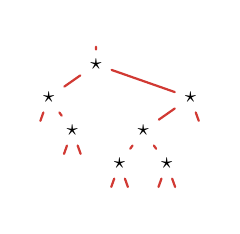
\begin{tikzpicture}[xscale=.15,yscale=.14,Centering]
        \node(0)at(0.00,-6.00){};
        \node(10)at(10.00,-12.00){};
        \node(12)at(12.00,-12.00){};
        \node(14)at(14.00,-6.00){};
        \node(2)at(2.00,-9.00){};
        \node(4)at(4.00,-9.00){};
        \node(6)at(6.00,-12.00){};
        \node(8)at(8.00,-12.00){};
        \node[NodeST](1)at(1.00,-3.00){\begin{math}\Product\end{math}};
        \node[NodeST](11)at(11.00,-9.00){\begin{math}\Product\end{math}};
        \node[NodeST](13)at(13.00,-3.00){\begin{math}\Product\end{math}};
        \node[NodeST](3)at(3.00,-6.00){\begin{math}\Product\end{math}};
        \node[NodeST](5)at(5.00,0.00){\begin{math}\Product\end{math}};
        \node[NodeST](7)at(7.00,-9.00){\begin{math}\Product\end{math}};
        \node[NodeST](9)at(9.00,-6.00){\begin{math}\Product\end{math}};
        \draw[Edge](0)--(1);
        \draw[Edge](1)--(5);
        \draw[Edge](10)--(11);
        \draw[Edge](11)--(9);
        \draw[Edge](12)--(11);
        \draw[Edge](13)--(5);
        \draw[Edge](14)--(13);
        \draw[Edge](2)--(3);
        \draw[Edge](3)--(1);
        \draw[Edge](4)--(3);
        \draw[Edge](6)--(7);
        \draw[Edge](7)--(9);
        \draw[Edge](8)--(7);
        \draw[Edge](9)--(13);
        \node(r)at(5.00,2.5){};
        \draw[Edge](r)--(5);
    \end{tikzpicture}
\end{equation}
is a partial composition in $\Mag$. This leads, by definition, to the
following complete composition maps of $\Mag$. Given $\Tfr \in \Mag(n)$
and $\Sfr_1, \dots, \Sfr_n \in \Mag$,
\begin{math}
    \Tfr \circ \left[\Sfr_1, \dots, \Sfr_n\right]
\end{math}
is the binary tree obtained by grafting simultaneously the roots of all
the $\Sfr_i$ onto the $i$th leaves of $\Tfr$. The unit of $\Mag$ is the
leaf. The number of binary trees of arity $n \geq 1$ is the $n$th
Catalan number $\Catalan(n)$ and hence, the Hilbert series of $\Mag$ is
\begin{equation}
    \HilbertSeries_{\Mag}(t)
    = \sum_{n \geq 1} \Catalan(n) t^n
    = \sum_{n \geq 1} \binom{2n - 1}{n - 1} \frac{1}{n} t^n.
\end{equation}
\medbreak

The operad $\Mag$ can be seen as the free operad generated by one binary
element~$\Product$. It satisfies the following universality property.
Let
\begin{math}
    \GeneratingSet := \GeneratingSet(2) := \left\{\Product'\right\}
\end{math}
be the graded set containing exactly one element $\Product'$ of arity
$2$. For any operad $\Oca$ and any map
\begin{math}
    f : \GeneratingSet(2) \to \Oca(2),
\end{math}
there exists a unique operad morphism $\phi : \Mag \to \Oca$ such that
$f = \phi \circ \Corolla$, where $\Corolla$ is the map sending
$\Product'$ to the unique binary tree of degree $1$ (and then, arity
$2$). In other terms, the diagram
\begin{equation}
    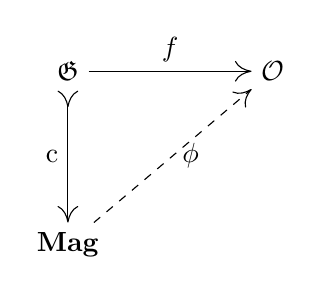
\begin{tikzpicture}[xscale=1.3,yscale=1.1,Centering]
        \node(G)at(0,0){\begin{math}\GeneratingSet\end{math}};
        \node(O)at(2,0){\begin{math}\Oca\end{math}};
        \node(AG)at(0,-2){\begin{math}\Mag\end{math}};
        \draw[Map](G)--(O)node[midway,above]{\begin{math}f\end{math}};
        \draw[Injection](G)--(AG)node[midway,left]
            {\begin{math}\Corolla\end{math}};
        \draw[Map,dashed](AG)--(O)node[midway,right]
            {\begin{math}\phi\end{math}};
    \end{tikzpicture}
\end{equation}
commutes.
\medbreak

We now provide some useful tools about binary trees. Given a binary tree
$\Tfr$, we denote by $ \PrefixWord(\Tfr)$ the \Def{prefix word} of
$\Tfr$, that is the word on $\{\Zero, \Two\}$ obtained by a left to
right depth-first traversal of $\Tfr$ and by writing $\Zero$ (resp.
$\Two$) when a leaf (resp. an internal node) is encountered. For
instance,
\begin{equation}
    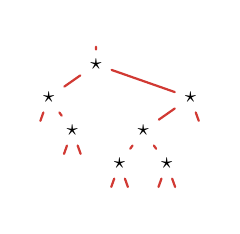
\begin{tikzpicture}[xscale=.15,yscale=.14,Centering]
        \node(0)at(0.00,-6.00){};
        \node(10)at(10.00,-12.00){};
        \node(12)at(12.00,-12.00){};
        \node(14)at(14.00,-6.00){};
        \node(2)at(2.00,-9.00){};
        \node(4)at(4.00,-9.00){};
        \node(6)at(6.00,-12.00){};
        \node(8)at(8.00,-12.00){};
        \node[NodeST](1)at(1.00,-3.00){\begin{math}\Product\end{math}};
        \node[NodeST](11)at(11.00,-9.00){\begin{math}\Product\end{math}};
        \node[NodeST](13)at(13.00,-3.00){\begin{math}\Product\end{math}};
        \node[NodeST](3)at(3.00,-6.00){\begin{math}\Product\end{math}};
        \node[NodeST](5)at(5.00,0.00){\begin{math}\Product\end{math}};
        \node[NodeST](7)at(7.00,-9.00){\begin{math}\Product\end{math}};
        \node[NodeST](9)at(9.00,-6.00){\begin{math}\Product\end{math}};
        \draw[Edge](0)--(1);
        \draw[Edge](1)--(5);
        \draw[Edge](10)--(11);
        \draw[Edge](11)--(9);
        \draw[Edge](12)--(11);
        \draw[Edge](13)--(5);
        \draw[Edge](14)--(13);
        \draw[Edge](2)--(3);
        \draw[Edge](3)--(1);
        \draw[Edge](4)--(3);
        \draw[Edge](6)--(7);
        \draw[Edge](7)--(9);
        \draw[Edge](8)--(7);
        \draw[Edge](9)--(13);
        \node(r)at(5.00,2.5){};
        \draw[Edge](r)--(5);
    \end{tikzpicture}
    \enspace \xmapsto{\; \PrefixWord \;} \enspace
    \Two \Two \Zero \Two \Zero \Zero \Two \Two \Two \Zero \Zero \Two
    \Zero \Zero \Zero.
\end{equation}
The set of all the words on $\{\Zero, \Two\}$ is endowed with the
lexicographic order $\leq$ induced by $\Zero < \Two$. By extension, this
defines a total order on each set $\Mag(n)$, $n \geq 1$. Indeed, we set
$\Tfr \leq \Tfr'$ if $\Tfr$ and $\Tfr'$ have the same arity and
$\PrefixWord(\Tfr) \leq \PrefixWord(\Tfr')$. Let also the
\Def{left rank} of $\Tfr$ as the number $\LRank(\Tfr)$ of internal
nodes in the left branch beginning at the root of $\Tfr$. For instance,
\begin{equation}
    \begin{tikzpicture}[xscale=.15,yscale=.14,Centering]
        \node(0)at(0.00,-9.00){};
        \node(10)at(10.00,-9.00){};
        \node(12)at(12.00,-9.00){};
        \node(14)at(14.00,-9.00){};
        \node(2)at(2.00,-12.00){};
        \node(4)at(4.00,-12.00){};
        \node(6)at(6.00,-6.00){};
        \node(8)at(8.00,-9.00){};
        \node[NodeST](1)at(1.00,-6.00){\begin{math}\Product\end{math}};
        \node[NodeST](11)at(11.00,-3.00){\begin{math}\Product\end{math}};
        \node[NodeST](13)at(13.00,-6.00){\begin{math}\Product\end{math}};
        \node[NodeST](3)at(3.00,-9.00){\begin{math}\Product\end{math}};
        \node[NodeST](5)at(5.00,-3.00){\begin{math}\Product\end{math}};
        \node[NodeST](7)at(7.00,0.00){\begin{math}\Product\end{math}};
        \node[NodeST](9)at(9.00,-6.00){\begin{math}\Product\end{math}};
        \draw[Edge](0)--(1);
        \draw[Edge](1)--(5);
        \draw[Edge](10)--(9);
        \draw[Edge](11)--(7);
        \draw[Edge](12)--(13);
        \draw[Edge](13)--(11);
        \draw[Edge](14)--(13);
        \draw[Edge](2)--(3);
        \draw[Edge](3)--(1);
        \draw[Edge](4)--(3);
        \draw[Edge](5)--(7);
        \draw[Edge](6)--(5);
        \draw[Edge](8)--(9);
        \draw[Edge](9)--(11);
        \node(r)at(7.00,2.25){};
        \draw[Edge](r)--(7);
    \end{tikzpicture}
    \enspace \xmapsto{\; \LRank\; } \enspace 3.
\end{equation}
Equivalently, $\LRank(\Tfr)$ is the length of the prefix of
$\PrefixWord(\Tfr)$ containing only the letter $\Two$. A binary tree
$\Sfr$ is a \Def{subtree} of $\Tfr$ if it possible to stack $\Sfr$ onto
$\Tfr$ by possibly superimposing leaves of $\Sfr$ onto internal nodes of
$\Tfr$. More formally, by using the operad $\Mag$ and its composition
maps, this is equivalent to the fact that $\Tfr$ expresses as
\begin{equation}
    \Tfr = \Rfr \circ_i
    \left(\Sfr \circ \left[\Rfr_1, \dots, \Rfr_n\right]\right)
\end{equation}
where $\Rfr$ and $\Rfr_1$, \dots, $\Rfr_n$ are binary trees,
$i \in [|\Rfr|]$, and $n$ is the arity of $\Sfr$. When, on the contrary,
$\Sfr$ is not a subtree of $\Tfr$, we say that $\Tfr$ \Def{avoids}
$\Sfr$.
\medbreak

%%%%%%%%%%%%%%%%%%%%%%%%%%%%%%%%%%%%%%%%%%%%%%%%%%%%%%%%%%%%%%%%%%%%%%%%
%%%%%%%%%%%%%%%%%%%%%%%%%%%%%%%%%%%%%%%%%%%%%%%%%%%%%%%%%%%%%%%%%%%%%%%%
\subsection{Rewrite systems on binary trees}
We present here notions about rewrite systems on binary trees. General
notations and notions appear in~\cite{BN98}.
\medbreak

A \Def{rewrite rule} is an ordered pair $(\Sfr, \Sfr')$ of binary trees
such that $|\Sfr| = |\Sfr'|$. A set $S$ of rewrite rules is a binary
relation on $\Mag$ and it shall be denoted by $\Rew$. We denote by
$\Sfr \Rew \Sfr'$ the fact that $(\Sfr, \Sfr') \in \Rew$. In the sequel,
to define a set of rewrite rules $\Rew$, we shall simply list all the
pairs $\Sfr \Rew \Sfr'$ contained in $\Rew$. The \Def{degree}
$\Deg(\Rew)$ of $\Rew$ is the maximal degree of the binary trees in
relation through $\Rew$. Note that $\Deg(\Rew)$ can be not defined when
$\Rew$ is infinite.
\medbreak

If $\Rew$ is a set of rewrite rules, we denote by $\RewContext$ the
\Def{rewrite relation induced} by $\Rew$. Formally we have
\begin{equation} \label{equ:rewrite_relation_induced}
    \Tfr \circ_i
    \left(\Sfr \circ \left[\Rfr_1, \dots, \Rfr_{n}\right]\right)
    \RewContext
    \Tfr \circ_i
    \left(\Sfr' \circ \left[\Rfr_1, \dots, \Rfr_{n}\right]\right),
\end{equation}
if $\Sfr \Rew \Sfr'$ where $n = |\Sfr|$, and $\Tfr$, $\Rfr_1$, \dots,
$\Rfr_n$ are binary trees. In other words, one has
$\Tfr \RewContext \Tfr'$ if it is possible to obtain $\Tfr'$ from $\Tfr$
by replacing a subtree $\Sfr$ of $\Tfr$ by $\Sfr'$ whenever
$\Sfr \Rew \Sfr'$. For instance, if $\Rew$ is the set of rewrite rules
containing the single rewrite rule
\begin{equation} \label{equ:example_rewrite_rule}
    \begin{tikzpicture}[xscale=.22,yscale=.22,Centering]
        \node(0)at(0.00,-3.50){};
        \node(2)at(2.00,-5.25){};
        \node(4)at(4.00,-5.25){};
        \node(6)at(6.00,-1.75){};
        \node[NodeST](1)at(1.00,-1.75){\begin{math}\Product\end{math}};
        \node[NodeST](3)at(3.00,-3.50){\begin{math}\Product\end{math}};
        \node[NodeST](5)at(5.00,0.00){\begin{math}\Product\end{math}};
        \draw[Edge](0)--(1);
        \draw[EdgeColorF](1)--(5);
        \draw[Edge](2)--(3);
        \draw[EdgeColorF](3)--(1);
        \draw[Edge](4)--(3);
        \draw[Edge](6)--(5);
        \node(r)at(5.00,1.31){};
        \draw[Edge](r)--(5);
    \end{tikzpicture}
    \enspace \Rew \enspace
    \begin{tikzpicture}[xscale=.22,yscale=.22,Centering]
        \node(0)at(0.00,-1.75){};
        \node(2)at(2.00,-3.50){};
        \node(4)at(4.00,-5.25){};
        \node(6)at(6.00,-5.25){};
        \node[NodeST](1)at(1.00,0.00){\begin{math}\Product\end{math}};
        \node[NodeST](3)at(3.00,-1.75){\begin{math}\Product\end{math}};
        \node[NodeST](5)at(5.00,-3.50){\begin{math}\Product\end{math}};
        \draw[Edge](0)--(1);
        \draw[Edge](2)--(3);
        \draw[EdgeColorF](3)--(1);
        \draw[Edge](4)--(5);
        \draw[EdgeColorF](5)--(3);
        \draw[Edge](6)--(5);
        \node(r)at(1.00,1.31){};
        \draw[Edge](r)--(1);
    \end{tikzpicture}\,,
\end{equation}
one has
\begin{equation} \label{equ:example_rewrite_step}
    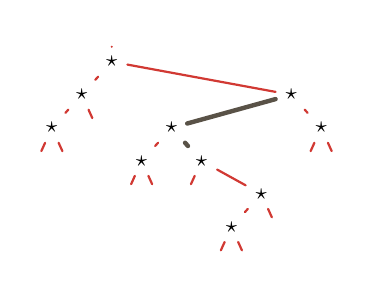
\begin{tikzpicture}[xscale=.19,yscale=.14,Centering]
        \node(0)at(0.00,-9.00){};
        \node(10)at(10.00,-12.00){};
        \node(12)at(12.00,-18.00){};
        \node(14)at(14.00,-18.00){};
        \node(16)at(16.00,-15.00){};
        \node(18)at(18.00,-9.00){};
        \node(2)at(2.00,-9.00){};
        \node(20)at(20.00,-9.00){};
        \node(4)at(4.00,-6.00){};
        \node(6)at(6.00,-12.00){};
        \node(8)at(8.00,-12.00){};
        \node[NodeST](1)at(1.00,-6.00){\begin{math}\Product\end{math}};
        \node[NodeST](11)at(11.00,-9.00)
            {\begin{math}\Product\end{math}};
        \node[NodeST](13)at(13.00,-15.00)
            {\begin{math}\Product\end{math}};
        \node[NodeST](15)at(15.00,-12.00)
            {\begin{math}\Product\end{math}};
        \node[NodeST](17)at(17.00,-3.00)
            {\begin{math}\Product\end{math}};
        \node[NodeST](19)at(19.00,-6.00)
            {\begin{math}\Product\end{math}};
        \node[NodeST](3)at(3.00,-3.00){\begin{math}\Product\end{math}};
        \node[NodeST](5)at(5.00,0.00){\begin{math}\Product\end{math}};
        \node[NodeST](7)at(7.00,-9.00){\begin{math}\Product\end{math}};
        \node[NodeST](9)at(9.00,-6.00){\begin{math}\Product\end{math}};
        \draw[Edge](0)--(1);
        \draw[Edge](1)--(3);
        \draw[Edge](10)--(11);
        \draw[EdgeColorF](11)--(9);
        \draw[Edge](12)--(13);
        \draw[Edge](13)--(15);
        \draw[Edge](14)--(13);
        \draw[Edge](15)--(11);
        \draw[Edge](16)--(15);
        \draw[Edge](17)--(5);
        \draw[Edge](18)--(19);
        \draw[Edge](19)--(17);
        \draw[Edge](2)--(1);
        \draw[Edge](20)--(19);
        \draw[Edge](3)--(5);
        \draw[Edge](4)--(3);
        \draw[Edge](6)--(7);
        \draw[Edge](7)--(9);
        \draw[Edge](8)--(7);
        \draw[EdgeColorF](9)--(17);
        \node(r)at(5.00,2.25){};
        \draw[Edge](r)--(5);
    \end{tikzpicture}
    \enspace \RewContext \enspace
    \begin{tikzpicture}[xscale=.19,yscale=.14,Centering]
        \node(0)at(0.00,-9.00){};
        \node(10)at(10.00,-9.00){};
        \node(12)at(12.00,-18.00){};
        \node(14)at(14.00,-18.00){};
        \node(16)at(16.00,-15.00){};
        \node(18)at(18.00,-15.00){};
        \node(2)at(2.00,-9.00){};
        \node(20)at(20.00,-15.00){};
        \node(4)at(4.00,-6.00){};
        \node(6)at(6.00,-9.00){};
        \node(8)at(8.00,-9.00){};
        \node[NodeST](1)at(1.00,-6.00){\begin{math}\Product\end{math}};
        \node[NodeST](11)at(11.00,-6.00)
            {\begin{math}\Product\end{math}};
        \node[NodeST](13)at(13.00,-15.00)
            {\begin{math}\Product\end{math}};
        \node[NodeST](15)at(15.00,-12.00)
            {\begin{math}\Product\end{math}};
        \node[NodeST](17)at(17.00,-9.00)
            {\begin{math}\Product\end{math}};
        \node[NodeST](19)at(19.00,-12.00)
            {\begin{math}\Product\end{math}};
        \node[NodeST](3)at(3.00,-3.00){\begin{math}\Product\end{math}};
        \node[NodeST](5)at(5.00,0.00){\begin{math}\Product\end{math}};
        \node[NodeST](7)at(7.00,-6.00){\begin{math}\Product\end{math}};
        \node[NodeST](9)at(9.00,-3.00){\begin{math}\Product\end{math}};
        \draw[Edge](0)--(1);
        \draw[Edge](1)--(3);
        \draw[Edge](10)--(11);
        \draw[EdgeColorF](11)--(9);
        \draw[Edge](12)--(13);
        \draw[Edge](13)--(15);
        \draw[Edge](14)--(13);
        \draw[Edge](15)--(17);
        \draw[Edge](16)--(15);
        \draw[EdgeColorF](17)--(11);
        \draw[Edge](18)--(19);
        \draw[Edge](19)--(17);
        \draw[Edge](2)--(1);
        \draw[Edge](20)--(19);
        \draw[Edge](3)--(5);
        \draw[Edge](4)--(3);
        \draw[Edge](6)--(7);
        \draw[Edge](7)--(9);
        \draw[Edge](8)--(7);
        \draw[Edge](9)--(5);
        \node(r)at(5.00,2.25){};
        \draw[Edge](r)--(5);
    \end{tikzpicture}\,.
\end{equation}
The right member of~\eqref{equ:example_rewrite_step} is obtained by
replacing, in the tree of left member
of~\eqref{equ:example_rewrite_step}, a subtree equal to the left
member of~\eqref{equ:example_rewrite_rule} starting at the right child
of its root by the right member of~\eqref{equ:example_rewrite_rule}.
\medbreak

Let $\Rew$ be a set of rewrite rules and $\RewContext$ be the rewrite
relation induced by $\Rew$. Since $\RewContext$ is in particular a
binary relation on $\Mag$, the classical notations about closures apply
here: we denote by $\RewContextT$ (resp. $\RewContextRT$,
$\RewContextRST$) the transitive (resp. reflexive and transitive,
reflexive, symmetric, and transitive) closure of $\RewContext$.
\medbreak

When $\Tfr_0$, $\Tfr_1$, \dots, $\Tfr_k$ are binary trees such that
\begin{equation}
    \Tfr_0 \RewContext \Tfr_1 \RewContext \cdots \RewContext \Tfr_k,
\end{equation}
we say that $\Tfr_0$ is \Def{rewritable} by $\RewContext$ into $\Tfr_k$
in $k$ \Def{steps}. When there is no infinite chain
\begin{equation} \label{equ:infinite_chain}
    \Tfr_0 \RewContext \Tfr_1 \RewContext \Tfr_2 \RewContext \cdots
\end{equation}
we say that $\RewContext$ is terminating. To establish the termination
of a rewrite relation, we will use the following criterion.
\medbreak

\begin{Lemma}\label{lem:prefix_word_termination}
    Let $\Rew$ be a set of rewrite rules on $\Mag$. If for any
    $\Tfr, \Tfr' \in \Mag$ such that $\Tfr \Rew \Tfr'$ one has
    $\Tfr > \Tfr'$, then the rewrite relation induced by $\Rew$ is
    terminating.
\end{Lemma}
\begin{proof}
    Observe first that for any binary trees $\Tfr$ and $\Sfr$, the
    prefix word of $\Tfr \circ_i \Sfr$ is obtained by replacing the
    $i$th $\Zero$ of $\PrefixWord(\Tfr)$ by $\PrefixWord(\Sfr)$. For
    this reason, and due to the
    definition~\eqref{equ:complete_composition} of $\circ$, for any
    binary trees $\Sfr$ and $\Rfr_1, \dots, \Rfr_n$ where $n$ is the
    arity of $\Sfr$, the prefix word of
    $\Sfr \circ \left[\Rfr_1, \dots, \Rfr_n\right]$ is obtained by
    replacing from right to left each $\Zero$ of $\PrefixWord(\Sfr)$ by
    the prefix words of each $\Rfr_i$. This, together with the
    definition~\eqref{equ:rewrite_relation_induced} of the rewrite
    relation $\RewContext$ induced by $\Rew$ and the hypothesis of the
    statement of the lemma, implies that if $\Tfr$ and $\Tfr'$ are two
    binary trees such that $\Tfr \RewContext \Tfr'$,
    $\PrefixWord(\Tfr) > \PrefixWord\left(\Tfr'\right)$. This leads to
    the fact that any chain
    \begin{math}
        \Tfr_0 \Rew \Tfr_1 \Rew \Tfr_2 \Rew \cdots
    \end{math}
    is finite since
    \begin{math}
        \Tfr_0 > \Tfr_1 > \Tfr_2 > \cdots
    \end{math}
    and there is a finite number of binary trees of a fixed arity.
    Therefore, $\RewContext$ is terminating.
\end{proof}
\medbreak

A \Def{normal form} for $\RewContext$ is a binary tree $\Tfr$ such
that for all binary trees $\Tfr'$, $\Tfr \RewContextRT \Tfr'$ implies
$\Tfr' = \Tfr$. In other words, a normal form for $\RewContext$ is a
tree which is not rewritable by $\RewContext$. A normal form for
$\RewContext$ of a binary tree $\Tfr$ is a normal form $\overline{\Tfr}$
for $\RewContext$ such that $\Tfr\RewContextRT\overline{\Tfr}$. When no
confusion is possible, we simply say normal form instead of normal form
for $\RewContext$. The set of all the normal forms is denoted by
$\NormalForms_{\RewContext}$. The trees of $\NormalForms_{\RewContext}$
admit the following description, useful for enumerative prospects.
\medbreak

\begin{Lemma} \label{lem:normal_forms_avoiding}
    Let $\Rew$ be a set of rewrite rules on $\Mag$ and $\RewContext$ be
    the rewrite relation induced by $\Rew$. Then,
    $\NormalForms_{\RewContext}$ is the set of all the binary trees that
    avoid all the trees appearing as left members of~$\Rew$.
\end{Lemma}
\begin{proof}
    Assume first that $\Tfr$ is a binary tree avoiding all the trees
    appearing as left members of~$\Rew$. Then, due to the
    definition~\eqref{equ:rewrite_relation_induced} of $\RewContext$,
    $\Tfr$ is not rewritable by $\RewContext$. Hence, $\Tfr$ is a normal
    form for $\RewContext$. Conversely, assume that
    $\Tfr \in \NormalForms_{\RewContext}$. In this case, by definition
    of a normal form, $\Tfr$ is not rewritable by $\RewContext$, so that
    $\Tfr$ does not admit any occurrence of a tree appearing as a left
    member of~$\Rew$.
\end{proof}
\medbreak

When for all binary trees $\Tfr$, $\Sfr_1$, and $\Sfr_2$ such that
$\Tfr \RewContextRT \Sfr_1$ and $\Tfr \RewContextRT \Sfr_2$, there
exists a binary tree $\Tfr'$ such that $\Sfr_1 \RewContextRT \Tfr'$ and
$\Sfr_2 \RewContextRT \Tfr'$, we say that $\RewContext$ is
\Def{confluent}. Besides, a tree $\Tfr$ is a \Def{branching tree} for
$\RewContext$ if there exists two different trees $\Sfr_1$ and $\Sfr_2$
satisfying $\Tfr \RewContext \Sfr_1$ and $\Tfr \RewContext \Sfr_2$. In
this case, the pair $\{\Sfr_1, \Sfr_2\}$ is a \Def{branching pair} for
$\Tfr$. Moreover, the branching pair $\{\Sfr_1, \Sfr_2\}$ is
\Def{joinable} if there exists a binary tree $\Tfr'$ such that
$\Sfr_1 \RewContextRT \Tfr'$ and $\Sfr_2 \RewContextRT \Tfr'$. The
diamond lemma~\cite{New42} is based upon the inspection of the branching
pairs of a terminating rewrite relation $\RewContext$ in order to prove
its confluence.
\medbreak

\begin{Lemma} \label{lem:diamond_lemma}
    Let $\Rew$ be a set of rewrite rules on $\Mag$ and $\RewContext$ be
    the rewrite relation induced by $\Rew$. Then, if $\RewContext$ is
    terminating and all its branching pairs are joinable, $\RewContext$
    is convergent.
\end{Lemma}
\medbreak

When $\RewContext$ is terminating and confluent, $\RewContext$ is said
\Def{convergent}. We shall use the following result to prove that
a terminating rewrite relation is convergent.
\medbreak

\begin{Lemma} \label{lem:degree_confluence}
    Let $\Rew$ be a set of rewrite rules on $\Mag$ having a degree
    $\Deg(\Rew)$. Then, if the rewrite relation $\RewContext$ induced by
    $\Rew$ is terminating and all its branching pairs made of trees of
    degrees at most $2 \, \Deg(\Rew) - 1$ are joinable, $\RewContext$ is
    convergent.
\end{Lemma}
\begin{proof}
    The statement of the lemma is the specialization on rewrite
    relations on $\Mag$ of a more general result about rewrite relations
    on trees contained in~\cite{Gir16}.
\end{proof}
\medbreak

Let us now go back on operads. Let $\Congr$ be an operad congruence of
$\Mag$. If $\Tfr$ is a binary tree, we denote by $[\Tfr]_{\Congr}$ the
$\Congr$-equivalence class of $\Tfr$. By definition, $[\Tfr]_{\Congr}$
is an element of the quotient operad
\begin{equation} \label{equ:quotient_operad_mag}
    \Oca := \Mag/_{\Congr}.
\end{equation}
A set of rewrite rules $\Rew$ on $\Mag$ is an \Def{orientation} of
$\Congr$ if $\RewContextRST$ and $\Congr$ are equal as binary relations,
where $\RewContext$ is the rewrite relation induced by $\Rew$. Moreover,
$\Rew$ is a \Def{convergent} (resp. \Def{terminating}, \Def{confluent})
orientation of $\Congr$ if $\RewContext$ is convergent (resp.
terminating, confluent). A \Def{presentation} of the quotient operad
$\Oca$ of the form~\eqref{equ:quotient_operad_mag} is the data of a
generating set for the operad congruence $\Congr$. Observe that
any orientation of $\Congr$ is a presentation of $\Oca$, so that the
above nomenclature (\Def{convergent}, \Def{terminating}, and
\Def{confluent}) still holds for presentations. A presentation is said
to be \Def{finite} if it is a finite set.
\medbreak

When $\Rew$ is a convergent orientation of $\Congr$, the set
$\NormalForms_{\RewContext}$ of all normal forms of $\RewContext$ is
called a \Def{Poincaré-Birkhoff-Witt basis} (or a \Def{PBW basis} for
short) of the quotient operad $\Oca$ (see~\cite{Hof10,DK10}). This forms
a one-to-one correspondence between the sets
$\NormalForms_{\RewContext}(n)$ and $\Oca(n)$, $n \geq 1$. In other
words, a PBW basis offers a way to assign with each $\Congr$-equivalence
class $[\Tfr]_{\Congr}$ a representative
\begin{math}
    \Tfr' \in [\Tfr]_{\Congr} \cap \NormalForms_{\RewContext}.
\end{math}
A \Def{combinatorial realization} of an operad $\Oca$ of the
form~\eqref{equ:quotient_operad_mag} is an operad $\Cca$ isomorphic to
$\Oca$ which admits an explicit description of its elements and an
explicit description of its partial composition maps. The knowledge of a
PBW basis $\Cca := \NormalForms_{\RewContext}$ of $\Oca$ provides a
combinatorial realization $\Cca$ of $\Oca$. Indeed, the partial
composition $\Tfr' \circ_i \Sfr'$ of two binary trees $\Tfr'$ and
$\Sfr'$ of $\Cca$ is the tree obtained by grafting the root of $\Sfr'$
onto the $i$th leaf of $\Tfr'$ and by rewriting by $\RewContext$ this
tree as much as possible in order to obtain a normal form. This process
is well-defined since, by hypothesis, $\RewContext$ is convergent.
\medbreak

When $\Rew$ is a terminating but not convergent orientation of $\Congr$,
we shall use a variant of the \Def{Buchberger semi-algorithm} for
operads~\cite[Section 3.7]{DK10} to compute a set of rewrite rules
$\Rew'$ such that, as binary relations $\Rew \subseteq \Rew'$, and
$\Rew'$ is a convergent orientation of $\Congr$. This semi-algorithm
takes as input a finite set of rewrite rules $\Rew$ and outputs the set
of rewrite rules $\Rew'$ satisfying the property stated above. Here is,
step by step, a description of its execution:
\begin{enumerate}[label={(\it\arabic*)}]
    \item Set $\Rew' := \Rew$ and let $\BranchingTrees$ be the set of
    branching trees for $\RewContext$.
    \smallbreak

    \item \label{item:loop_start_buchberger}
    If $\BranchingTrees$ is empty, the execution stops and the output
    is $\Rew'$.
    \smallbreak

    \item\label{item:choice_branching_tree} Otherwise, let $\Tfr$ be a
    branching tree for $\RewContext'$. Remove $\Tfr$ from
    $\BranchingTrees$.
    \smallbreak

    \item\label{item:choice_branching_pair} Let $\{\Sfr_1, \Sfr_2\}$ be
    a branching pair for $\Tfr$.
    \smallbreak

    \item\label{item:computed_normal_forms} Let $\bar{\Sfr_1}$ and
    $\bar{\Sfr_2}$ be normal forms of $\Sfr_1$ and $\Sfr_2$,
    respectively.
    \smallbreak

    \item \label{item:new_rewrite_rule_buchberger}
    If $\bar{\Sfr_1}$ is different from $\bar{\Sfr_2}$, add
    to $\Rew'$ the rewrite rule
    \begin{math}
        \max_\leq \left\{\bar{\Sfr_1}, \bar{\Sfr_2}\right\}
        \Rew'
        \min_\leq \left\{\bar{\Sfr_1}, \bar{\Sfr_2}\right\}.
    \end{math}
    \smallbreak

    \item Add to $\BranchingTrees$ all new branching trees of degrees at
    most $2 \Deg(\Rew') - 1$ created by the rewrite rule created in
    Step~\ref{item:new_rewrite_rule_buchberger}.
    \smallbreak

    \item Go to Step~\ref{item:loop_start_buchberger}.
\end{enumerate}
The set of rewrite rules $\Rew'$ outputted by this semi-algorithm is a
\Def{completion} of $\Rew$. By Lemma~\ref{lem:degree_confluence},
$\RewContext'$ is confluent. Notice that, for certain inputs $\Rew$,
this semi-algorithm never stops. Notice also that the computed
completion depend on the total order $\leq$ on the binary trees of a
same arity, the choices at Steps~\ref{item:choice_branching_tree}
and~\ref{item:choice_branching_pair} as well as the computed normal
forms at Step~\ref{item:computed_normal_forms}.
\medbreak

\Todo{S: je crois qu'il faudrait préciser les choix que l'on fait aux
étapes (3), (4) et (5).}


%%%%%%%%%%%%%%%%%%%%%%%%%%%%%%%%%%%%%%%%%%%%%%%%%%%%%%%%%%%%%%%%%%%%%%%%
%%%%%%%%%%%%%%%%%%%%%%%%%%%%%%%%%%%%%%%%%%%%%%%%%%%%%%%%%%%%%%%%%%%%%%%%
%%%%%%%%%%%%%%%%%%%%%%%%%%%%%%%%%%%%%%%%%%%%%%%%%%%%%%%%%%%%%%%%%%%%%%%%
\section{Magmatic operads}


%%%%%%%%%%%%%%%%%%%%%%%%%%%%%%%%%%%%%%%%%%%%%%%%%%%%%%%%%%%%%%%%%%%%%%%%
%%%%%%%%%%%%%%%%%%%%%%%%%%%%%%%%%%%%%%%%%%%%%%%%%%%%%%%%%%%%%%%%%%%%%%%%
%%%%%%%%%%%%%%%%%%%%%%%%%%%%%%%%%%%%%%%%%%%%%%%%%%%%%%%%%%%%%%%%%%%%%%%%
%%%%%%%%%%%%%%%%%%%%%%%%%%%%%%%%%%%%%%%%%%%%%%%%%%%%%%%%%%%%%%%%%%%%%%%%
%%%%%%%%%%%%%%%%%%%%%%%%%%%%%%%%%%%%%%%%%%%%%%%%%%%%%%%%%%%%%%%%%%%%%%%%
%%%%%%%%%%%%%%%%%%%%%%%%%%%%%%%%%%%%%%%%%%%%%%%%%%%%%%%%%%%%%%%%%%%%%%%%
\section{Generalizations of the associative operad}
\label{sec:CAs_d}

In this section, we define comb associative operads and we show that the
set of such operads admits a lattice structure, isomorphic to the
lattice division for nonnegative integers. We relate this lattice to the
lattice of linear magmatic quotients. We also provide a finite
convergent presentation of the comb associative operad corresponding
to~$3$.
\medbreak

%%%%%%%%%%%%%%%%%%%%%%%%%%%%%%%%%%%%%%%%%%%%%%%%%%%%%%%%%%%%%%%%%%%%%%%%
%%%%%%%%%%%%%%%%%%%%%%%%%%%%%%%%%%%%%%%%%%%%%%%%%%%%%%%%%%%%%%%%%%%%%%%%
\subsection{Comb associative operads}
Recall first that the \Def{associative operad} $\As$ is the quotient
of $\Mag$ by the smallest operad congruence $\Congr$ satisfying
\begin{equation}
    \begin{tikzpicture}[xscale=.24,yscale=.24,Centering]
        \node(0)at(0.00,-3.33){};
        \node(2)at(2.00,-3.33){};
        \node(4)at(4.00,-1.67){};
        \node[NodeST](1)at(1.00,-1.67)
            {\begin{math}\Product\end{math}};
        \node[NodeST](3)at(3.00,0.00)
            {\begin{math}\Product\end{math}};
        \draw[Edge](0)--(1);
        \draw[Edge](1)--(3);
        \draw[Edge](2)--(1);
        \draw[Edge](4)--(3);
        \node(r)at(3.00,1.5){};
        \draw[Edge](r)--(3);
    \end{tikzpicture}
    \Congr
    \begin{tikzpicture}[xscale=.24,yscale=.24,Centering]
        \node(0)at(0.00,-1.67){};
        \node(2)at(2.00,-3.33){};
        \node(4)at(4.00,-3.33){};
        \node[NodeST](1)at(1.00,0.00)
                {\begin{math}\Product\end{math}};
        \node[NodeST](3)at(3.00,-1.67)
                {\begin{math}\Product\end{math}};
        \draw[Edge](0)--(1);
        \draw[Edge](2)--(3);
        \draw[Edge](3)--(1);
        \draw[Edge](4)--(3);
        \node(r)at(1.00,1.5){};
        \draw[Edge](r)--(1);
    \end{tikzpicture}\,.
\end{equation}
We propose here a generalization of $\Congr$ in order to define
generalizations of $\As$.
\medbreak

Let, for any integer $\gamma \geq 1$, the binary trees $\LComb{\gamma}$
and $\RComb{\gamma}$ be respectively the left and the right combs of
degree $\gamma$. These trees are depicted as
\begin{equation}
    \LComb{\gamma} = \enspace
    \begin{tikzpicture}[xscale=.26,yscale=.3,Centering]
        \node(0)at(0.00,-5.25){};
        \node(2)at(2.00,-5.25){};
        \node(4)at(4.00,-3.50){};
        \node(6)at(6.00,-1.75){};
        \node[NodeST](1)at(1.00,-3.50){\begin{math}\Product\end{math}};
        \node[NodeST](3)at(3.00,-1.75){\begin{math}\Product\end{math}};
        \node[NodeST](5)at(5.00,0.00){\begin{math}\Product\end{math}};
        \draw[Edge](0)--(1);
        \draw[Edge,dotted](1)edge[]node[font=\tiny]{
            \begin{math}\gamma\! -\! 1\end{math}\hspace*{.6cm}}(3);
        \draw[Edge](2)--(1);
        \draw[Edge](3)--(5);
        \draw[Edge](4)--(3);
        \draw[Edge](6)--(5);
        \node(r)at(5.00,1.5){};
        \draw[Edge](r)--(5);
    \end{tikzpicture}
    \qquad \mbox{and} \qquad
    \RComb{\gamma} =
    \begin{tikzpicture}[xscale=.26,yscale=.3,Centering]
        \node(0)at(0.00,-1.75){};
        \node(2)at(2.00,-3.50){};
        \node(4)at(4.00,-5.25){};
        \node(6)at(6.00,-5.25){};
        \node[NodeST](1)at(1.00,0.00){\begin{math}\Product\end{math}};
        \node[NodeST](3)at(3.00,-1.75){\begin{math}\Product\end{math}};
        \node[NodeST](5)at(5.00,-3.50){\begin{math}\Product\end{math}};
        \draw[Edge](0)--(1);
        \draw[Edge](2)--(3);
        \draw[Edge](3)--(1);
        \draw[Edge](4)--(5);
        \draw[Edge,dotted](5)edge[]node[font=\tiny]{
            \hspace*{.6cm}\begin{math}\gamma\! -\! 1\end{math}}(3);
        \draw[Edge](6)--(5);
        \node(r)at(1.00,1.5){};
        \draw[Edge](r)--(1);
    \end{tikzpicture}\,,
\end{equation}
where the values on the dotted edges denote the number of internal
nodes they contain. We shall employ this drawing convention in the
sequel, combined with the convention stipulating that dotted edges
with no value have any number of internal nodes. Let us now define for
any $\gamma \geq 1$ the \Def{$\gamma$-comb associative operad}
$\CAs{\gamma}$ as the quotient operad $\Mag/_{\CongrCAs{\gamma}}$ where
$\CongrCAs{\gamma}$ is the smallest operad congruence of $\Mag$
satisfying
\begin{equation} \label{equ:congruence_CAs_gamma}
    \LComb{\gamma} \enspace \CongrCAs{\gamma} \enspace \RComb{\gamma}.
\end{equation}
Notice that $\CongrCAs{1}$ is trivial so that
$\CAs{1} = \Mag$, and that $\CongrCAs{2}$ is the operad congruence
defining $\As$ so that $\CAs{2} = \As$. Let also
\begin{equation}
    \CAsAll := \left\{\CAs{\gamma} : \gamma\geq 1\right\}
\end{equation}
be the set of all the $\gamma$-comb associative operads.
\medbreak

%%%%%%%%%%%%%%%%%%%%%%%%%%%%%%%%%%%%%%%%%%%%%%%%%%%%%%%%%%%%%%%%%%%%%%%
%%%%%%%%%%%%%%%%%%%%%%%%%%%%%%%%%%%%%%%%%%%%%%%%%%%%%%%%%%%%%%%%%%%%%%%
\subsection{Lattice of comb associative operads}
In order to introduce a lattice structure on $\CAsAll$, we begin by
studying operad morphisms between its elements by mean of intermediate
lemmas.
\medbreak

\begin{Lemma} \label{lem:first_dimensions_CAs}
    For all positive integers $\gamma$ and $n$ such that $\gamma \geq 2$
    and $n \leq \gamma + 1$,
    \begin{equation}
        \# \CAs{\gamma}(n) =
        \begin{cases}
            \Catalan(n)
                & \mbox{ if } n \leq \gamma, \\
            \Catalan(\gamma + 1) - 1
                & \mbox{ otherwise } (n = \gamma + 1).
        \end{cases}
    \end{equation}
\end{Lemma}
\begin{proof}
    Since the equivalence relation $\CongrCAs{\gamma}$ is trivial on the
    binary trees of degrees $d < \gamma$, and since a binary tree of
    degree $d$ has arity $n := d + 1$, one has
    $\# \CAs{\gamma}(n) = \# \Mag(n) = \Catalan(n)$ with
    $n \leq \gamma$. Besides, by definition of $\CongrCAs{\gamma}$, all
    the $\CongrCAs{\gamma}$-equivalence classes of binary trees of
    degree $\gamma$ are trivial, except one consisting in the pair
    $\left\{\LComb{\gamma}, \RComb{\gamma}\right\}$. Therefore, since a
    binary tree of degree $d$ has arity $n := \gamma + 1$,
    \begin{math}
        \# \CAs{\gamma}(n)
        = \# \Mag(\gamma + 1) - 1
        = \Catalan(\gamma + 1) - 1.
    \end{math}
\end{proof}
\medbreak

\begin{Lemma} \label{lem:surjective_morphisms_CAs}
    Let $\gamma$ and $\gamma'$ be two positive integers. If there exists
    an operad morphism $\varphi:\CAs{\gamma'} \to \CAs{\gamma}$, then it
    is surjective and unique.
\end{Lemma}
\begin{proof}
    The operad $\CAs{\gamma'}$ is generated by one binary generator
    $[\Product]_{\CongrCAs{\gamma'}}$, which is the image of the binary
    generator $\Product$ of $\Mag$ in $\CAs{\gamma'}$. Hence, $\varphi$
    is entirely determined by the image
    $\varphi\left([\Product]_{\CongrCAs{\gamma'}}\right)$. Moreover,
    $\varphi([\Product]_{\CongrCAs{\gamma'}})$ has to be of arity $2$ in
    $\CAs{\gamma}$, so that we necessarily have
    \begin{math}
        \varphi\left([\Product]_{\CongrCAs{\gamma'}}\right)
        =
        [\Product]_{\CongrCAs{\gamma}}.
    \end{math}
    Hence, if $\varphi$ exists, it is the unique operad morphism from
    $\CAs{\gamma'}$ to $\CAs{\gamma}$ determined by the previous formula.
    In this case, $[\Product]_{\CongrCAs{\gamma}}$ being in the image of
    $\varphi$, the latter is surjective.
\end{proof}
\medbreak

\begin{Lemma} \label{lem:injective_morphisms_CAs}
    Let $\gamma$ and $\gamma'$ be two positive integers and
    $\varphi:\CAs{\gamma'} \to \CAs{\gamma}$ be an operad morphism.
    Then, $\varphi$ is injective if and only if $\gamma = \gamma'$.
\end{Lemma}
\begin{proof}
    Assume that $\varphi$ is injective. By
    Lemma~\ref{lem:surjective_morphisms_CAs}, $\varphi$ is also
    surjective, so that $\varphi$ is an isomorphism. If
    $\gamma \ne \gamma'$, by Lemma~\ref{lem:first_dimensions_CAs}, there
    is a positive integer $n$ such that
    $\# \CAs{\gamma}(n) \ne \# \CAs{\gamma'}(n)$. This is contradictory
    with the fact that $\CAs{\gamma}$ and $\CAs{\gamma'}$ are
    isomorphic. Hence, $\gamma = \gamma'$.
    \smallbreak

    Conversely, if $\gamma = \gamma'$, the only operad morphism from
    $\CAs{\gamma}$ to itself sends the generator
    $[\Product]_{\CongrCAs{\gamma}}$ to itself. This maps extends as
    an operad morphism into the identity morphism which is of course
    injective.
\end{proof}
\medbreak

\begin{Lemma} \label{lem:morphism_CAs}
    Let $\gamma$ and $\gamma'$ be two positive integers. There exists an
    operad morphism $\varphi:\CAs{\gamma'} \to \CAs{\gamma}$ if and only
    if
    \begin{math}
      \LComb{\gamma'} \CongrCAs{\gamma} \RComb{\gamma'}.
    \end{math}
\end{Lemma}
\begin{proof}
    Assume that $\varphi:\CAs{\gamma'} \to \CAs{\gamma}$ is an operad
    morphism. By Lemma~\ref{lem:surjective_morphisms_CAs}, $\varphi$
    satisfies
    \begin{math}
        \varphi\left(\left[\Tfr\right]_{\CongrCAs{\gamma'}}\right)
        = \left[\Tfr\right]_{\CongrCAs{\gamma}}
    \end{math}
    for any binary tree $\Tfr$.
    Since
    \begin{math}
        \varphi\left(
        \left[\LComb{\gamma'}\right]_{\CongrCAs{\gamma'}}
        \right)
        =
        \varphi\left(
        \left[\RComb{\gamma'}\right]_{\CongrCAs{\gamma'}}
        \right),
    \end{math}
    we have
    \begin{math}
        \left[\LComb{\gamma'}\right]_{\CongrCAs{\gamma}}
        =
        \left[\RComb{\gamma'}\right]_{\CongrCAs{\gamma}},
    \end{math}
    which is equivalent to the fact that
    \begin{math}
        \LComb{\gamma'} \CongrCAs{\gamma} \RComb{\gamma'}.
    \end{math}
    \smallbreak

    Conversely, when
    \begin{math}
        \LComb{\gamma'}\CongrCAs{\gamma}\RComb{\gamma'},
    \end{math}
    let $\varphi:\CAs{\gamma'}(2) \to \CAs{\gamma}(2)$ be the map
    defined by
    \begin{math}
        \varphi\left(
        \left[\Product\right]_{\CongrCAs{\gamma'}}\right)
        :=
        \left[\Product\right]_{\CongrCAs{\gamma}}.
    \end{math}
    Now, since $\CongrCAs{\gamma}$ is coarser than $\CongrCAs{\gamma'}$,
    $\varphi$ extends (in a unique way) into an operad morphism, whence
    the statement of the lemma.
\end{proof}
\medbreak

We define the binary relation $\OrdCAs$ on $\CAsAll$ as follows: we have
$\CAs{\gamma} \OrdCAs \CAs{\gamma'}$ if and only if there exists a
morphism $\varphi:\CAs{\gamma'} \to \CAs{\gamma}$.
\medbreak

\begin{Proposition}\label{prop:poset_CAs}
    The binary relation $\OrdCAs$ is a partial order relation on
    $\CAsAll$.
\end{Proposition}
\begin{proof}
    The binary relation $\OrdCAs$ is reflexive since there exists the
    identity morphism of $\CAs{\gamma}$ for every positive integer
    $\gamma$. Let us now assume that
    $\varphi:\CAs{\gamma''} \to \CAs{\gamma'}$ and
    $\psi:\CAs{\gamma'} \to \CAs{\gamma}$ are two operad morphisms. By
    Lemma~\ref{lem:morphism_CAs}, one has
    $\LComb{\gamma''} \CongrCAs{\gamma'} \RComb{\gamma''}$ and
    $\LComb{\gamma'} \CongrCAs{\gamma} \RComb{\gamma'}$. This implies
    that $\CongrCAs{\gamma}$ is coarser than $\CongrCAs{\gamma'}$ and
    that $\CongrCAs{\gamma'}$ is coarser that $\CongrCAs{\gamma''}$. Now,
    again by Lemma~\ref{lem:morphism_CAs}, $\psi \circ \varphi$ is an
    operad morphism. Hence, $\OrdCAs$ is transitive. Finally, let us
    assume that there exist morphisms
    $\varphi:\CAs{\gamma'}\to\CAs{\gamma}$ and
    $\psi:\CAs{\gamma}\to\CAs{\gamma'}$. In particular,
    $\psi \circ \varphi$ and $\varphi \circ \psi$ are endomorphisms of
    $\CAs{\gamma'}$ and $\CAs{\gamma}$, respectively. From
    Lemma~\ref{lem:surjective_morphisms_CAs}, these two morphisms are
    identity morphisms, so that $\varphi$ and $\psi$ are injective. From
    Lemma~\ref{lem:injective_morphisms_CAs}, $\gamma$ and $\gamma'$ are
    equal, which proves that $\OrdCAs$ is anti-symmetric. Hence,
    $\OrdCAs$ is a partial order.
\end{proof}
\medbreak

In order to show that $\left(\CAsAll, \OrdCAs\right)$ extends into a
lattice, we relate $\left(\CAsAll, \OrdCAs\right)$ with the lattice of
integers $\left(\N,\mid, \gcd, \lcm\right)$, where $\mid$ denotes the
division relation, $\gcd$ denotes the greatest common divisor, and
$\lcm$ the least common multiple operators, respectively.
\medbreak

Recall that $\LRank(\Tfr)$ denotes the left rank of a binary tree
$\Tfr$, defined in Section~\ref{sec:operad_Mag}. Besides, to simplify
the notation, we shall write $\bar{a}$ instead of $a - 1$ for any
integer~$a$.
\medbreak

\begin{Lemma}\label{lem:left_rank_and_CongrCAs}
    Let $\gamma$ be a positive integer and let $\Tfr$ and
    $\Tfr'$ be two binary trees. If $\Tfr \CongrCAs{\gamma} \Tfr'$, then
    \begin{equation}
        \LRank(\Tfr) \pmod{\bar{\gamma}}
        \enspace = \enspace
        \LRank\left(\Tfr'\right) \pmod{\bar{\gamma}}.
    \end{equation}
\end{Lemma}
\begin{proof}
  We consider the rewrite rule $\LComb{\gamma} \Rew \RComb{\gamma}$
    on $\Mag$. First, we show that
    \begin{equation} \label{eq:rewriting_invariant}
        \Tfr \RewContext \Tfr'
        \mbox{ implies }
        \LRank\left(\Tfr'\right) \pmod{\bar{\gamma}} = \LRank\left(\Tfr\right)
        \, \pmod{\bar{\gamma}}.
    \end{equation}
    Indeed, for all $\Tfr \in \Mag$, let
    $\Tfr_1, \dots, \Tfr_{\LRank\left(\Tfr\right)}$ be the binary trees
    such that
    \begin{math}
      \Tfr =
       \LComb{\LRank\left(\Tfr\right)} \circ
      \left[\, \Leaf \, \Tfr_1, \dots,
      \Tfr_{\LRank\left(\Tfr\right)} \right].
    \end{math}
    Thus, if $\Tfr \RewContext \Tfr'$, then one of the following two
    cases occurs:
    \begin{enumerate}[label={(\it\roman*)}]
    \item the rewrite step is applied on one of the trees $\Tfr_i$,
      that is there exists $\Tfr_i'$ such that
            \begin{math}
              \Tfr' = \LComb{\LRank\left(\Tfr\right)} \circ
              \left[\, \Leaf ,\Tfr_1, \dots, \Tfr_i',\dots,
                    \Tfr_{\LRank\left(\Tfr\right)}
              \right] \mbox{, so that }
              \LRank\left(\Tfr'\right) = \LRank\left(\Tfr\right);
            \end{math}
          \item the rewrite step is applied in the left branch beginning
            at the root, that is there exists $i$ such that
            \begin{math}
              \Tfr' = \LComb{\LRank\left(\Tfr\right)-\bar{\gamma}} \circ
              \left[ \Leaf ,\Tfr_1, \dots,
                 \RComb{\bar{\gamma}} \circ
                 [\Tfr_{i},\dots, \Tfr_{i+\bar{\gamma}}]
                 ,\dots, \Tfr_{\LRank\left(\Tfr\right)}
              \right]
              \mbox{, so that }\\
              \LRank\left(\Tfr'\right) =
              \LRank\left(\Tfr\right) - \bar{\gamma} =
              \LRank\left(\Tfr\right) \pmod{\bar{\gamma}}
            \end{math}.
    \end{enumerate}
    This concludes the proof of~\eqref{eq:rewriting_invariant}.
    \smallbreak

    We deduce from~\eqref{eq:rewriting_invariant} that the equivalence
    relation $\simeq$ defined by
    \begin{equation}
        \Tfr \simeq \Tfr' \mbox{ if and only if }
        \LRank\left(\Tfr'\right) \pmod{\bar{\gamma}} =
        \LRank\left(\Tfr\right) \, \pmod{\bar{\gamma}}
    \end{equation}
    contains the relation $\RewContext$, so that it contains its
    transitive symmetric closure. The latter is $\CongrCAs{\gamma}$,
    which concludes the proof of Lemma~\ref{lem:left_rank_and_CongrCAs}.
\end{proof}
\medbreak

\begin{Proposition} \label{prop:division_CAs}
    Let $\gamma$ and $\gamma'$ be two positive integers. Then, there
    exists a morphism $\varphi:\CAs{\gamma'} \to \CAs{\gamma}$ if and
    only if $\bar{\gamma} \mid \bar{\gamma'}$.
\end{Proposition}
\begin{proof}
    From Lemma~\ref{lem:morphism_CAs}, it is enough to show that
    $\LComb{\gamma'} \CongrCAs{\gamma} \RComb{\gamma'}$ if and only if
    $\bar{\gamma} \mid \bar{\gamma'}$. If
    $\LComb{\gamma'}\CongrCAs{\gamma}\RComb{\gamma'}$, $\gamma$ is
    smaller than $\gamma'$ (this is a consequence of the existence of a
    surjective morphism $\varphi:\CAs{\gamma'} \to \CAs{\gamma}$ and
    Lemma~\ref{lem:first_dimensions_CAs}). From
    Lemma~\ref{lem:left_rank_and_CongrCAs}, we deduce that
    \begin{math}
        \LRank\left(\LComb{\gamma'}\right)
        - \LRank\left(\RComb{\gamma'}\right)
        = \bar{\gamma'}
    \end{math}
    is divisible by $\bar{\gamma}$, which shows the direct implication.
    \smallbreak

    Conversely, if
    $\bar{\gamma} \mid \bar{\gamma'}$, the rewrite
    rule $\LComb{\gamma} \Rew \RComb{\gamma}$ induces the
    sequence
    \begin{multline}
        \LComb{\gamma'} \enspace = \enspace
        \begin{tikzpicture}[xscale=.19,yscale=.25,Centering]
            \node(0)at(0.00,-13.12){};
            \node(10)at(10.00,-5.62){};
            \node(12)at(12.00,-3.75){};
            \node(14)at(14.00,-1.88){};
            \node(2)at(2.00,-13.12){};
            \node(4)at(4.00,-11.25){};
            \node(6)at(6.00,-9.38){};
            \node(8)at(8.00,-7.50){};
            \node[NodeST](1)at(1.00,-11.25)
                {\begin{math}\Product\end{math}};
            \node[NodeST](11)at(11.00,-1.88)
                {\begin{math}\Product\end{math}};
            \node[NodeST](13)at(13.00,0.00)
                {\begin{math}\Product\end{math}};
            \node[NodeST](3)at(3.00,-9.38)
                {\begin{math}\Product\end{math}};
            \node[NodeST](5)at(5.00,-7.50)
                {\begin{math}\Product\end{math}};
            \node[NodeST](7)at(7.00,-5.62)
                {\begin{math}\Product\end{math}};
            \node[NodeST](9)at(9.00,-3.75)
                {\begin{math}\Product\end{math}};
            \draw[Edge](0)--(1);
            \draw[Edge,dotted](1)edge[]node[font=\footnotesize]{
                \begin{math}\bar{\gamma}\end{math}\hspace*{.5cm}}(3);
            \draw[Edge](10)--(9);
            \draw[Edge](11)--(13);
            \draw[Edge](12)--(11);
            \draw[Edge](14)--(13);
            \draw[Edge](2)--(1);
            \draw[Edge,dotted](3)--(5);
            \draw[Edge](4)--(3);
            \draw[Edge,dotted](5)edge[]node[font=\footnotesize]{
                \begin{math}\bar{\gamma}\end{math}\hspace*{.5cm}}(7);
            \draw[Edge](6)--(5);
            \draw[Edge](7)--(9);
            \draw[Edge](8)--(7);
            \draw[Edge,dotted](9)edge[]node[font=\footnotesize]{
                \begin{math}\bar{\gamma}\end{math}\hspace*{.5cm}}(11);
            \node(r)at(13.00,1.41){};
            \draw[Edge](r)--(13);
        \end{tikzpicture}
        \enspace \RewContext \enspace
        \begin{tikzpicture}[xscale=.19,yscale=.2,Centering]
            \node(0)at(0.00,-12.50){};
            \node(10)at(10.00,-5.00){};
            \node(12)at(12.00,-7.50){};
            \node(14)at(14.00,-7.50){};
            \node(2)at(2.00,-12.50){};
            \node(4)at(4.00,-10.00){};
            \node(6)at(6.00,-7.50){};
            \node(8)at(8.00,-5.00){};
            \node[NodeST](1)at(1.00,-10.00)
                {\begin{math}\Product\end{math}};
            \node[NodeST](11)at(11.00,-2.50)
                {\begin{math}\Product\end{math}};
            \node[NodeST](13)at(13.00,-5.00)
                {\begin{math}\Product\end{math}};
            \node[NodeST](3)at(3.00,-7.50)
                {\begin{math}\Product\end{math}};
            \node[NodeST](5)at(5.00,-5.00)
                {\begin{math}\Product\end{math}};
            \node[NodeST](7)at(7.00,-2.50)
                {\begin{math}\Product\end{math}};
            \node[NodeST](9)at(9.00,0.00)
                {\begin{math}\Product\end{math}};
            \draw[Edge](0)--(1);
            \draw[Edge,dotted](1)edge[]node[font=\footnotesize]{
                \begin{math}\bar{\gamma}\end{math}\hspace*{.5cm}}(3);
            \draw[Edge](10)--(11);
            \draw[Edge](11)--(9);
            \draw[Edge](12)--(13);
            \draw[Edge,dotted](13)edge[]node[font=\footnotesize]{
                \hspace*{.5cm}\begin{math}\bar{\gamma}\end{math}}(11);
            \draw[Edge](14)--(13);
            \draw[Edge](2)--(1);
            \draw[Edge,dotted](3)--(5);
            \draw[Edge](4)--(3);
            \draw[Edge,dotted](5)edge[]node[font=\footnotesize]{
                \begin{math}\bar{\gamma}\end{math}\hspace*{.5cm}}(7);
            \draw[Edge](6)--(5);
            \draw[Edge](7)--(9);
            \draw[Edge](8)--(7);
            \node(r)at(9.00,1.88){};
            \draw[Edge](r)--(9);
        \end{tikzpicture} \\
        \enspace \RewContext \enspace
        \begin{tikzpicture}[xscale=.19,yscale=.2,Centering]
            \node(0)at(0.00,-7.50){};
            \node(10)at(10.00,-10.00){};
            \node(12)at(12.00,-12.50){};
            \node(14)at(14.00,-12.50){};
            \node(2)at(2.00,-7.50){};
            \node(4)at(4.00,-5.00){};
            \node(6)at(6.00,-5.00){};
            \node(8)at(8.00,-7.50){};
            \node[NodeST](1)at(1.00,-5.00)
                {\begin{math}\Product\end{math}};
            \node[NodeST](11)at(11.00,-7.50)
                {\begin{math}\Product\end{math}};
            \node[NodeST](13)at(13.00,-10.00)
                {\begin{math}\Product\end{math}};
            \node[NodeST](3)at(3.00,-2.50)
                {\begin{math}\Product\end{math}};
            \node[NodeST](5)at(5.00,0.00)
                {\begin{math}\Product\end{math}};
            \node[NodeST](7)at(7.00,-2.50)
                {\begin{math}\Product\end{math}};
            \node[NodeST](9)at(9.00,-5.00)
                {\begin{math}\Product\end{math}};
            \draw[Edge](0)--(1);
            \draw[Edge,dotted](1)edge[]node[font=\footnotesize]{
                \begin{math}\bar{\gamma}\end{math}\hspace*{.5cm}}(3);
            \draw[Edge](10)--(11);
            \draw[Edge](11)--(9);
            \draw[Edge](12)--(13);
            \draw[Edge,dotted](13)edge[]node[font=\footnotesize]{
                \hspace*{.5cm}\begin{math}\bar{\gamma}\end{math}}(11);
            \draw[Edge](14)--(13);
            \draw[Edge](2)--(1);
            \draw[Edge,dotted](3)--(5);
            \draw[Edge](4)--(3);
            \draw[Edge](6)--(7);
            \draw[Edge](7)--(5);
            \draw[Edge](8)--(9);
            \draw[Edge,dotted](9)edge[]node[font=\footnotesize]{
                \hspace*{.5cm}\begin{math}\bar{\gamma}\end{math}}(7);
            \node(r)at(5.00,1.88){};
            \draw[Edge](r)--(5);
        \end{tikzpicture}
        \enspace \RewContextRT \enspace
        \begin{tikzpicture}[xscale=.19,yscale=.25,Centering]
            \node(0)at(0.00,-1.88){};
            \node(10)at(10.00,-11.25){};
            \node(12)at(12.00,-13.12){};
            \node(14)at(14.00,-13.12){};
            \node(2)at(2.00,-3.75){};
            \node(4)at(4.00,-5.62){};
            \node(6)at(6.00,-7.50){};
            \node(8)at(8.00,-9.38){};
            \node[NodeST](1)at(1.00,0.00)
                {\begin{math}\Product\end{math}};
            \node[NodeST](11)at(11.00,-9.38)
                {\begin{math}\Product\end{math}};
            \node[NodeST](13)at(13.00,-11.25)
                {\begin{math}\Product\end{math}};
            \node[NodeST](3)at(3.00,-1.88)
                {\begin{math}\Product\end{math}};
            \node[NodeST](5)at(5.00,-3.75)
                {\begin{math}\Product\end{math}};
            \node[NodeST](7)at(7.00,-5.62)
                {\begin{math}\Product\end{math}};
            \node[NodeST](9)at(9.00,-7.50)
                {\begin{math}\Product\end{math}};
            \draw[Edge](0)--(1);
            \draw[Edge](10)--(11);
            \draw[Edge,dotted](11)--(9);
            \draw[Edge](12)--(13);
            \draw[Edge,dotted](13)edge[]node[font=\footnotesize]{
                \hspace*{.5cm}\begin{math}\bar{\gamma}\end{math}}(11);
            \draw[Edge](14)--(13);
            \draw[Edge](2)--(3);
            \draw[Edge](3)--(1);
            \draw[Edge](4)--(5);
            \draw[Edge,dotted](5)edge[]node[font=\footnotesize]{
                \hspace*{.5cm}\begin{math}\bar{\gamma}\end{math}}(3);
            \draw[Edge](6)--(7);
            \draw[Edge](7)--(5);
            \draw[Edge](8)--(9);
            \draw[Edge,dotted](9)edge[]node[font=\footnotesize]{
                \hspace*{.5cm}\begin{math}\bar{\gamma}\end{math}}(7);
            \node(r)at(1.00,1.41){};
            \draw[Edge](r)--(1);
        \end{tikzpicture}
        \enspace = \enspace
        \RComb{\gamma'}
    \end{multline}
    of rewriting steps, where squared regions denotes left or right
    comb trees of degree $\gamma - 1$. Hence, we have
    $\LComb{\gamma'}\CongrCAs{\gamma}\RComb{\gamma'}$.
\end{proof}
\medbreak

Proposition~\ref{prop:division_CAs} implies the following result.
\medbreak

\begin{Theorem}\label{thm:lattice_CAs}
  The tuple $\LatCAs$ is a lattice, where $\InfCAs$ and $\SupCAs$ are
  defined, for all positive integers $\gamma$ and $\gamma'$, by
    \begin{equation}
      \CAs{\gamma}\InfCAs\CAs{\gamma'}
      :=\CAs{\gcd \left(\bar{\gamma}, \bar{\gamma'}\right)}
    \end{equation}
    and
    \begin{equation}
      \CAs{\gamma}\SupCAs\CAs{\gamma'}
      :=\CAs{\lcm \left(\bar{\gamma}, \bar{\gamma'}\right)}.
    \end{equation}
\end{Theorem}
\medbreak

The lattice $\left(\N, \mid, \gcd, \lcm\right)$ admits $1$ as minimum
element and $0$ as maximum element: any nonnegative integer is
divisible by $1$ and divides $0$. The corresponding property for
$\LatCAs$ is that it admits $\As=\CAs{2}$ as minimum element and $\Mag=
\CAs{1}$ as maximum element: any comb associative operad projects onto
$\As$ and is a quotient of $\Mag$.
\medbreak

We end this section by relating the lattice $\LatQMag$ introduced in
Section~\ref{sec:Magmatic_operads} with the lattice $\LatCAs$. As
explained in Section~\ref{sec:operad_Mag}, a set-theoretic operad can
be embedded into a linear operad, so that the operads $\CAs{\gamma}$ can
be embedded into quotient operads $\KCAs{\gamma}$ of $\KMag$. Formally,
the operad $\KCAs{\gamma}$ is equal to $\KMag/_{I_{\gamma}}$, where
$I_{\gamma}$ is the operadic ideal of $\KMag$ generated by
$\LComb{\gamma}-\RComb{\gamma}$. We obtain a new lattice $\LatKCAs$,
where $\KCAsAll$ is the set of all operads $\KCAs{\gamma}$. In this
linear framework, the condition $\KCAs{\gamma}\OrdCAs\KCAs{\gamma'}$
means that the dimension of the space
$\Hom\left(\KCAs{\gamma'},\KCAs{\gamma}\right)$ is equal to $1$. Hence,
$\LatKCAs$ is related to $\LatQMag$ by the following theorem.
\medbreak

\begin{Theorem} \label{thm:inclusion_lattice_CAs}
    The inclusion
    \begin{math}
        \iota:\left(\KCAsAll,\OrdCAs\right)
        \to
        \left(\QMag,\OrdQMag\right)
    \end{math}
    is nondecreasing. In particular, for all positive integers $\gamma$
    and $\gamma'$, we have
    \begin{equation} \label{equ:comparison_of_lattice_operations}
        \KCAs{\gcd \left(\bar{\gamma}, \bar{\gamma'}\right)}
        \OrdQMag
        \KCAs{\gamma}\InfQMag\KCAs{\gamma'}
    \end{equation}
    and
    \begin{equation}
        \KCAs{\gamma}\SupQMag\KCAs{\gamma'}
        \OrdQMag
        \KCAs{\lcm \left(\bar{\gamma}, \bar{\gamma'}\right)}.
    \end{equation}
\end{Theorem}
\medbreak

Note that $\LatKCAs$ does not embed as a sublattice of $\LatQMag$, that
is $\iota$ is not a lattice morphism. Consider for instance $\gamma = 3$
and $\gamma' = 4$, so that $\KCAs{\gamma} \InfCAs \KCAs{\gamma'}$ is
equal to $\KCAs{2} = \K\As$, whereas
$\KCAs{\gamma} \InfQMag \KCAs{\gamma'}$ is the quotient of $\KMag$ by the
two relations $\LComb{3} - \RComb{3}$ and $\LComb{4} - \RComb{4}$.
\medbreak

%%%%%%%%%%%%%%%%%%%%%%%%%%%%%%%%%%%%%%%%%%%%%%%%%%%%%%%%%%%%%%%%%%%%%%%%
%%%%%%%%%%%%%%%%%%%%%%%%%%%%%%%%%%%%%%%%%%%%%%%%%%%%%%%%%%%%%%%%%%%%%%%%
\subsection{Completion of comb associative operads}
We are now looking for finite convergent presentations of comb
associative operads. By definition, the operad $\CAs{\gamma}$ is the
quotient of $\Mag$ by the operad congruence spanned by the rewrite rule
\begin{equation} \label{equ:rew_1}
    \LComb{\gamma}
    \enspace \Rew \enspace
    \RComb{\gamma}\,.
\end{equation}
This rewrite rule is compatible with the lexicographic order on prefix
words presented at the beginning of Section~\ref{sec:operad_Mag} in the
sense that the prefix word of the left member of~\eqref{equ:rew_1} is
lexicographically greater than the prefix word of the right one.
\medbreak

However, the rewrite relation $\RewContext$ induced by $\Rew$ is not
confluent for $\gamma\geq 3$. Indeed, we have
\begin{equation} \label{equ:branching_pair_CAs_3}
    \LComb{\gamma+1}
    \enspace \RewContext \enspace
    \begin{tikzpicture}[xscale=.22,yscale=.20,Centering]
        \node(0)at(0.00,-4.50){};
        \node(2)at(2.00,-4.50){};
        \node(6)at(6.00,-6.75){};
        \node(8)at(8.00,-6.75){};
        \node[NodeST](1)at(1.00,-2.25){\begin{math}\Product\end{math}};
        \node[NodeST](3)at(3.00,0.00){\begin{math}\Product\end{math}};
        \node[NodeST](5)at(5.30,-1.4){\begin{math}\gamma\end{math}};
        \node[NodeST](7)at(7.00,-4.50){\begin{math}\Product\end{math}};
        \draw[Edge](0)--(1);
        \draw[Edge](1)--(3);
        \draw[Edge](2)--(1);
        \draw[Edge](6)--(7);
        \draw[Edge, dotted](7)--(3);
        \draw[Edge](8)--(7);
        \node(r)at(3.00,1.74){};
        \draw[Edge](r)--(3);
    \end{tikzpicture}
    \qquad \mbox{and} \qquad
    \LComb{\gamma+1}
    \enspace \RewContext \enspace
    \begin{tikzpicture}[xscale=.22,yscale=.22,Centering]
        \node(0)at(0.00,-3.60){};
        \node(4)at(4.00,-7.20){};
        \node(6)at(6.00,-7.20){};
        \node(8)at(8.00,-1.80){};
        \node[NodeST](1)at(1.00,-1.80){\begin{math}\Product\end{math}};
        \node[NodeST](3)at(3.25,-2.90){\begin{math}\gamma\end{math}};
        \node[NodeST](5)at(5.00,-5.40){\begin{math}\Product\end{math}};
        \node[NodeST](7)at(7.00,0.00){\begin{math}\Product\end{math}};
        \draw[Edge](0)--(1);
        \draw[Edge](1)--(7);
        \draw[Edge,dotted](5)--(1);
        \draw[Edge](4)--(5);
        \draw[Edge](6)--(5);
        \draw[Edge](8)--(7);
        \node(r)at(7.00,1.5){};
        \draw[Edge](r)--(7);
    \end{tikzpicture}\,,
\end{equation}
and the two right members of~\eqref{equ:branching_pair_CAs_3} form a
branching pair which is not joinable (since these two trees are
normal forms of $\RewContext$).
\medbreak

In order to transform the rewrite relation induced by~\eqref{equ:rew_1}
into a convergent one, we apply the Buchberger algorithm for
operads~\cite[Section 3.7]{DK10} with respect to the lexicographic order
on prefix words. We first focus on the special case $\gamma = 3$.
\medbreak

%%%%%%%%%%%%%%%%%%%%%%%%%%%%%%%%%%%%%%%%%%%%%%%%%%%%%%%%%%%%%%%%%%%%%%%%
\subsubsection{The \texorpdfstring{$3$}{3}-comb associative operad}
\label{subsubsec:CAs_3}

The Buchberger algorithm applied on binary trees of degrees $4$ to $7$
provides the new rewrite rules \smallbreak
\begin{minipage}{7cm}
\begin{equation} \label{equ:rew_2}
    \begin{tikzpicture}[xscale=.22,yscale=.22,Centering]
        \node(0)at(0.00,-3.60){};
        \node(2)at(2.00,-5.40){};
        \node(4)at(4.00,-7.20){};
        \node(6)at(6.00,-7.20){};
        \node(8)at(8.00,-1.80){};
        \node[NodeST](1)at(1.00,-1.80){\begin{math}\Product\end{math}};
        \node[NodeST](3)at(3.00,-3.60){\begin{math}\Product\end{math}};
        \node[NodeST](5)at(5.00,-5.40){\begin{math}\Product\end{math}};
        \node[NodeST](7)at(7.00,0.00){\begin{math}\Product\end{math}};
        \draw[Edge](0)--(1);
        \draw[Edge](1)--(7);
        \draw[Edge](2)--(3);
        \draw[Edge](3)--(1);
        \draw[Edge](4)--(5);
        \draw[Edge](5)--(3);
        \draw[Edge](6)--(5);
        \draw[Edge](8)--(7);
        \node(r)at(7.00,1.5){};
        \draw[Edge](r)--(7);
    \end{tikzpicture}
    \enspace \Rew \enspace
    \begin{tikzpicture}[xscale=.22,yscale=.20,Centering]
        \node(0)at(0.00,-4.50){};
        \node(2)at(2.00,-4.50){};
        \node(4)at(4.00,-4.50){};
        \node(6)at(6.00,-6.75){};
        \node(8)at(8.00,-6.75){};
        \node[NodeST](1)at(1.00,-2.25){\begin{math}\Product\end{math}};
        \node[NodeST](3)at(3.00,0.00){\begin{math}\Product\end{math}};
        \node[NodeST](5)at(5.00,-2.25){\begin{math}\Product\end{math}};
        \node[NodeST](7)at(7.00,-4.50){\begin{math}\Product\end{math}};
        \draw[Edge](0)--(1);
        \draw[Edge](1)--(3);
        \draw[Edge](2)--(1);
        \draw[Edge](4)--(5);
        \draw[Edge](5)--(3);
        \draw[Edge](6)--(7);
        \draw[Edge](7)--(5);
        \draw[Edge](8)--(7);
        \node(r)at(3.00,1.74){};
        \draw[Edge](r)--(3);
    \end{tikzpicture}
\end{equation}
\end{minipage},
\begin{minipage}{7cm}
\begin{equation} \label{equ:rew_3}
    \begin{tikzpicture}[xscale=.23,yscale=.21,Centering]
        \node(0)at(0.00,-1.83){};
        \node(10)at(10.00,-5.50){};
        \node(2)at(2.00,-3.67){};
        \node(4)at(4.00,-7.33){};
        \node(6)at(6.00,-9.17){};
        \node(8)at(8.00,-9.17){};
        \node[NodeST](1)at(1.00,0.00){\begin{math}\Product\end{math}};
        \node[NodeST](3)at(3.00,-1.83){\begin{math}\Product\end{math}};
        \node[NodeST](5)at(5.00,-5.50){\begin{math}\Product\end{math}};
        \node[NodeST](7)at(7.00,-7.33){\begin{math}\Product\end{math}};
        \node[NodeST](9)at(9.00,-3.67){\begin{math}\Product\end{math}};
        \draw[Edge](0)--(1);
        \draw[Edge](10)--(9);
        \draw[Edge](2)--(3);
        \draw[Edge](3)--(1);
        \draw[Edge](4)--(5);
        \draw[Edge](5)--(9);
        \draw[Edge](6)--(7);
        \draw[Edge](7)--(5);
        \draw[Edge](8)--(7);
        \draw[Edge](9)--(3);
        \node(r)at(1.00,1.75){};
        \draw[Edge](r)--(1);
    \end{tikzpicture}
    \enspace \Rew \enspace
    \begin{tikzpicture}[xscale=.22,yscale=.24,Centering]
        \node(0)at(0.00,-1.83){};
        \node(10)at(10.00,-9.17){};
        \node(2)at(2.00,-3.67){};
        \node(4)at(4.00,-5.50){};
        \node(6)at(6.00,-7.33){};
        \node(8)at(8.00,-9.17){};
        \node[NodeST](1)at(1.00,0.00){\begin{math}\Product\end{math}};
        \node[NodeST](3)at(3.00,-1.83){\begin{math}\Product\end{math}};
        \node[NodeST](5)at(5.00,-3.67){\begin{math}\Product\end{math}};
        \node[NodeST](7)at(7.00,-5.50){\begin{math}\Product\end{math}};
        \node[NodeST](9)at(9.00,-7.33){\begin{math}\Product\end{math}};
        \draw[Edge](0)--(1);
        \draw[Edge](10)--(9);
        \draw[Edge](2)--(3);
        \draw[Edge](3)--(1);
        \draw[Edge](4)--(5);
        \draw[Edge](5)--(3);
        \draw[Edge](6)--(7);
        \draw[Edge](7)--(5);
        \draw[Edge](8)--(9);
        \draw[Edge](9)--(7);
        \node(r)at(1.00,1.5){};
        \draw[Edge](r)--(1);
    \end{tikzpicture}
\end{equation}
\end{minipage},\\
\begin{minipage}{7cm}
\begin{equation}\label{equ:rew_4}
     \begin{tikzpicture}[xscale=.2,yscale=.19,Centering]
        \node(0)at(0.00,-2.20){};
        \node(10)at(10.00,-6.60){};
        \node(2)at(2.00,-6.60){};
        \node(4)at(4.00,-8.80){};
        \node(6)at(6.00,-8.80){};
        \node(8)at(8.00,-6.60){};
        \node[NodeST](1)at(1.00,0.00){\begin{math}\Product\end{math}};
        \node[NodeST](3)at(3.00,-4.40){\begin{math}\Product\end{math}};
        \node[NodeST](5)at(5.00,-6.60){\begin{math}\Product\end{math}};
        \node[NodeST](7)at(7.00,-2.20){\begin{math}\Product\end{math}};
        \node[NodeST](9)at(9.00,-4.40){\begin{math}\Product\end{math}};
        \draw[Edge](0)--(1);
        \draw[Edge](10)--(9);
        \draw[Edge](2)--(3);
        \draw[Edge](3)--(7);
        \draw[Edge](4)--(5);
        \draw[Edge](5)--(3);
        \draw[Edge](6)--(5);
        \draw[Edge](7)--(1);
        \draw[Edge](8)--(9);
        \draw[Edge](9)--(7);
        \node(r)at(1.00,2){};
        \draw[Edge](r)--(1);
    \end{tikzpicture}
    \enspace \Rew \enspace
    \begin{tikzpicture}[xscale=.22,yscale=.24,Centering]
        \node(0)at(0.00,-1.83){};
        \node(10)at(10.00,-9.17){};
        \node(2)at(2.00,-3.67){};
        \node(4)at(4.00,-5.50){};
        \node(6)at(6.00,-7.33){};
        \node(8)at(8.00,-9.17){};
        \node[NodeST](1)at(1.00,0.00){\begin{math}\Product\end{math}};
        \node[NodeST](3)at(3.00,-1.83){\begin{math}\Product\end{math}};
        \node[NodeST](5)at(5.00,-3.67){\begin{math}\Product\end{math}};
        \node[NodeST](7)at(7.00,-5.50){\begin{math}\Product\end{math}};
        \node[NodeST](9)at(9.00,-7.33){\begin{math}\Product\end{math}};
        \draw[Edge](0)--(1);
        \draw[Edge](10)--(9);
        \draw[Edge](2)--(3);
        \draw[Edge](3)--(1);
        \draw[Edge](4)--(5);
        \draw[Edge](5)--(3);
        \draw[Edge](6)--(7);
        \draw[Edge](7)--(5);
        \draw[Edge](8)--(9);
        \draw[Edge](9)--(7);
        \node(r)at(1.00,1.75){};
        \draw[Edge](r)--(1);
    \end{tikzpicture}
\end{equation}
\end{minipage}, 
\begin{minipage}{7cm}
\begin{equation} \label{equ:rew_5}
    \begin{tikzpicture}[xscale=.2,yscale=.2,Centering]
        \node(0)at(0.00,-2.17){};
        \node(10)at(10.00,-10.83){};
        \node(12)at(12.00,-10.83){};
        \node(2)at(2.00,-4.33){};
        \node(4)at(4.00,-8.67){};
        \node(6)at(6.00,-8.67){};
        \node(8)at(8.00,-8.67){};
        \node[NodeST](1)at(1.00,0.00){\begin{math}\Product\end{math}};
        \node[NodeST](11)at(11.00,-8.67)
            {\begin{math}\Product\end{math}};
        \node[NodeST](3)at(3.00,-2.17){\begin{math}\Product\end{math}};
        \node[NodeST](5)at(5.00,-6.50){\begin{math}\Product\end{math}};
        \node[NodeST](7)at(7.00,-4.33){\begin{math}\Product\end{math}};
        \node[NodeST](9)at(9.00,-6.50){\begin{math}\Product\end{math}};
        \draw[Edge](0)--(1);
        \draw[Edge](10)--(11);
        \draw[Edge](11)--(9);
        \draw[Edge](12)--(11);
        \draw[Edge](2)--(3);
        \draw[Edge](3)--(1);
        \draw[Edge](4)--(5);
        \draw[Edge](5)--(7);
        \draw[Edge](6)--(5);
        \draw[Edge](7)--(3);
        \draw[Edge](8)--(9);
        \draw[Edge](9)--(7);
        \node(r)at(1.00,1.75){};
        \draw[Edge](r)--(1);
    \end{tikzpicture}
    \Rew
    \begin{tikzpicture}[xscale=.21,yscale=.22,Centering]
        \node(0)at(0.00,-1.86){};
        \node(10)at(10.00,-11.14){};
        \node(12)at(12.00,-9.29){};
        \node(2)at(2.00,-3.71){};
        \node(4)at(4.00,-5.57){};
        \node(6)at(6.00,-7.43){};
        \node(8)at(8.00,-11.14){};
        \node[NodeST](1)at(1.00,0.00){\begin{math}\Product\end{math}};
        \node[NodeST](11)at(11.00,-7.43)
            {\begin{math}\Product\end{math}};
        \node[NodeST](3)at(3.00,-1.86){\begin{math}\Product\end{math}};
        \node[NodeST](5)at(5.00,-3.71){\begin{math}\Product\end{math}};
        \node[NodeST](7)at(7.00,-5.57){\begin{math}\Product\end{math}};
        \node[NodeST](9)at(9.00,-9.29){\begin{math}\Product\end{math}};
        \draw[Edge](0)--(1);
        \draw[Edge](10)--(9);
        \draw[Edge](11)--(7);
        \draw[Edge](12)--(11);
        \draw[Edge](2)--(3);
        \draw[Edge](3)--(1);
        \draw[Edge](4)--(5);
        \draw[Edge](5)--(3);
        \draw[Edge](6)--(7);
        \draw[Edge](7)--(5);
        \draw[Edge](8)--(9);
        \draw[Edge](9)--(11);
        \node(r)at(1.00,1.75){};
        \draw[Edge](r)--(1);
    \end{tikzpicture}
\end{equation}
\end{minipage},\\
\begin{minipage}{7cm}
\begin{equation} \label{equ:rew_6}
    \begin{tikzpicture}[xscale=.21,yscale=.21,Centering]
        \node(0)at(0.00,-2.17){};
        \node(10)at(10.00,-10.83){};
        \node(12)at(12.00,-10.83){};
        \node(2)at(2.00,-6.50){};
        \node(4)at(4.00,-6.50){};
        \node(6)at(6.00,-6.50){};
        \node(8)at(8.00,-8.67){};
        \node[NodeST](1)at(1.00,0.00){\begin{math}\Product\end{math}};
        \node[NodeST](11)at(11.00,-8.67)
            {\begin{math}\Product\end{math}};
        \node[NodeST](3)at(3.00,-4.33){\begin{math}\Product\end{math}};
        \node[NodeST](5)at(5.00,-2.17){\begin{math}\Product\end{math}};
        \node[NodeST](7)at(7.00,-4.33){\begin{math}\Product\end{math}};
        \node[NodeST](9)at(9.00,-6.50){\begin{math}\Product\end{math}};
        \draw[Edge](0)--(1);
        \draw[Edge](10)--(11);
        \draw[Edge](11)--(9);
        \draw[Edge](12)--(11);
        \draw[Edge](2)--(3);
        \draw[Edge](3)--(5);
        \draw[Edge](4)--(3);
        \draw[Edge](5)--(1);
        \draw[Edge](6)--(7);
        \draw[Edge](7)--(5);
        \draw[Edge](8)--(9);
        \draw[Edge](9)--(7);
        \node(r)at(1.00,1.75){};
        \draw[Edge](r)--(1);
    \end{tikzpicture}
    \Rew
    \begin{tikzpicture}[xscale=.22,yscale=.21,Centering]
        \node(0)at(0.00,-2.17){};
        \node(10)at(10.00,-10.83){};
        \node(12)at(12.00,-10.83){};
        \node(2)at(2.00,-4.33){};
        \node(4)at(4.00,-6.50){};
        \node(6)at(6.00,-10.83){};
        \node(8)at(8.00,-10.83){};
        \node[NodeST](1)at(1.00,0.00){\begin{math}\Product\end{math}};
        \node[NodeST](11)at(11.00,-8.67)
            {\begin{math}\Product\end{math}};
        \node[NodeST](3)at(3.00,-2.17){\begin{math}\Product\end{math}};
        \node[NodeST](5)at(5.00,-4.33){\begin{math}\Product\end{math}};
        \node[NodeST](7)at(7.00,-8.67){\begin{math}\Product\end{math}};
        \node[NodeST](9)at(9.00,-6.50){\begin{math}\Product\end{math}};
        \draw[Edge](0)--(1);
        \draw[Edge](10)--(11);
        \draw[Edge](11)--(9);
        \draw[Edge](12)--(11);
        \draw[Edge](2)--(3);
        \draw[Edge](3)--(1);
        \draw[Edge](4)--(5);
        \draw[Edge](5)--(3);
        \draw[Edge](6)--(7);
        \draw[Edge](7)--(9);
        \draw[Edge](8)--(7);
        \draw[Edge](9)--(5);
        \node(r)at(1.00,1.75){};
        \draw[Edge](r)--(1);
    \end{tikzpicture}\hspace{-8pt}
\end{equation}
\end{minipage},
\begin{minipage}{7cm}
\begin{equation} \label{equ:rew_7}
    \begin{tikzpicture}[xscale=.19,yscale=.17,Centering]
        \node(0)at(0.00,-5.20){};
        \node(10)at(10.00,-7.80){};
        \node(12)at(12.00,-7.80){};
        \node(2)at(2.00,-10.40){};
        \node(4)at(4.00,-10.40){};
        \node(6)at(6.00,-7.80){};
        \node(8)at(8.00,-5.20){};
        \node[NodeST](1)at(1.00,-2.60){\begin{math}\Product\end{math}};
        \node[NodeST](11)at(11.00,-5.20)
            {\begin{math}\Product\end{math}};
        \node[NodeST](3)at(3.00,-7.80){\begin{math}\Product\end{math}};
        \node[NodeST](5)at(5.00,-5.20){\begin{math}\Product\end{math}};
        \node[NodeST](7)at(7.00,0.00){\begin{math}\Product\end{math}};
        \node[NodeST](9)at(9.00,-2.60){\begin{math}\Product\end{math}};
        \draw[Edge](0)--(1);
        \draw[Edge](1)--(7);
        \draw[Edge](10)--(11);
        \draw[Edge](11)--(9);
        \draw[Edge](12)--(11);
        \draw[Edge](2)--(3);
        \draw[Edge](3)--(5);
        \draw[Edge](4)--(3);
        \draw[Edge](5)--(1);
        \draw[Edge](6)--(5);
        \draw[Edge](8)--(9);
        \draw[Edge](9)--(7);
        \node(r)at(7.00,2){};
        \draw[Edge](r)--(7);
    \end{tikzpicture}
    \enspace \Rew \enspace
        \begin{tikzpicture}[xscale=.2,yscale=.19,Centering]
        \node(0)at(0.00,-4.33){};
        \node(10)at(10.00,-10.83){};
        \node(12)at(12.00,-10.83){};
        \node(2)at(2.00,-4.33){};
        \node(4)at(4.00,-4.33){};
        \node(6)at(6.00,-6.50){};
        \node(8)at(8.00,-8.67){};
        \node[NodeST](1)at(1.00,-2.17){\begin{math}\Product\end{math}};
        \node[NodeST](11)at(11.00,-8.67)
            {\begin{math}\Product\end{math}};
        \node[NodeST](3)at(3.00,0.00){\begin{math}\Product\end{math}};
        \node[NodeST](5)at(5.00,-2.17){\begin{math}\Product\end{math}};
        \node[NodeST](7)at(7.00,-4.33){\begin{math}\Product\end{math}};
        \node[NodeST](9)at(9.00,-6.50){\begin{math}\Product\end{math}};
        \draw[Edge](0)--(1);
        \draw[Edge](1)--(3);
        \draw[Edge](10)--(11);
        \draw[Edge](11)--(9);
        \draw[Edge](12)--(11);
        \draw[Edge](2)--(1);
        \draw[Edge](4)--(5);
        \draw[Edge](5)--(3);
        \draw[Edge](6)--(7);
        \draw[Edge](7)--(5);
        \draw[Edge](8)--(9);
        \draw[Edge](9)--(7);
        \node(r)at(3.00,1.75){};
        \draw[Edge](r)--(3);
    \end{tikzpicture}\hspace{-10pt}
\end{equation}
\end{minipage},\\
\begin{minipage}{7cm}
\begin{equation} \label{equ:rew_8}
    \begin{tikzpicture}[xscale=.2,yscale=.19,Centering]
        \node(0)at(0.00,-2.14){};
        \node(10)at(10.00,-12.86){};
        \node(12)at(12.00,-12.86){};
        \node(14)at(14.00,-12.86){};
        \node(2)at(2.00,-4.29){};
        \node(4)at(4.00,-6.43){};
        \node(6)at(6.00,-8.57){};
        \node(8)at(8.00,-12.86){};
        \node[NodeST](1)at(1.00,0.00){\begin{math}\Product\end{math}};
        \node[NodeST](11)at(11.00,-8.57)
            {\begin{math}\Product\end{math}};
        \node[NodeST](13)at(13.00,-10.71)
            {\begin{math}\Product\end{math}};
        \node[NodeST](3)at(3.00,-2.14){\begin{math}\Product\end{math}};
        \node[NodeST](5)at(5.00,-4.29){\begin{math}\Product\end{math}};
        \node[NodeST](7)at(7.00,-6.43){\begin{math}\Product\end{math}};
        \node[NodeST](9)at(9.00,-10.71){\begin{math}\Product\end{math}};
        \draw[Edge](0)--(1);
        \draw[Edge](10)--(9);
        \draw[Edge](11)--(7);
        \draw[Edge](12)--(13);
        \draw[Edge](13)--(11);
        \draw[Edge](14)--(13);
        \draw[Edge](2)--(3);
        \draw[Edge](3)--(1);
        \draw[Edge](4)--(5);
        \draw[Edge](5)--(3);
        \draw[Edge](6)--(7);
        \draw[Edge](7)--(5);
        \draw[Edge](8)--(9);
        \draw[Edge](9)--(11);
        \node(r)at(1.00,2){};
        \draw[Edge](r)--(1);
    \end{tikzpicture}
    \hspace{-10pt}\Rew
    \begin{tikzpicture}[xscale=.22,yscale=.2,Centering]
        \node(0)at(0.00,-1.88){};
        \node(10)at(10.00,-13.12){};
        \node(12)at(12.00,-13.12){};
        \node(14)at(14.00,-11.25){};
        \node(2)at(2.00,-3.75){};
        \node(4)at(4.00,-5.62){};
        \node(6)at(6.00,-7.50){};
        \node(8)at(8.00,-9.38){};
        \node[NodeST](1)at(1.00,0.00){\begin{math}\Product\end{math}};
        \node[NodeST](11)at(11.00,-11.25)
            {\begin{math}\Product\end{math}};
        \node[NodeST](13)at(13.00,-9.38)
            {\begin{math}\Product\end{math}};
        \node[NodeST](3)at(3.00,-1.88){\begin{math}\Product\end{math}};
        \node[NodeST](5)at(5.00,-3.75){\begin{math}\Product\end{math}};
        \node[NodeST](7)at(7.00,-5.62){\begin{math}\Product\end{math}};
        \node[NodeST](9)at(9.00,-7.50){\begin{math}\Product\end{math}};
        \draw[Edge](0)--(1);
        \draw[Edge](10)--(11);
        \draw[Edge](11)--(13);
        \draw[Edge](12)--(11);
        \draw[Edge](13)--(9);
        \draw[Edge](14)--(13);
        \draw[Edge](2)--(3);
        \draw[Edge](3)--(1);
        \draw[Edge](4)--(5);
        \draw[Edge](5)--(3);
        \draw[Edge](6)--(7);
        \draw[Edge](7)--(5);
        \draw[Edge](8)--(9);
        \draw[Edge](9)--(7);
        \node(r)at(1.00,2){};
        \draw[Edge](r)--(1);
    \end{tikzpicture}\hspace{-20pt}
\end{equation}
\end{minipage},
\begin{minipage}{7cm}
\begin{equation} \label{equ:rew_9}
    \begin{tikzpicture}[xscale=0.18,yscale=.2,Centering]
        \node(0)at(0.00,-2.14){};
        \node(10)at(10.00,-12.86){};
        \node(12)at(12.00,-12.86){};
        \node(14)at(14.00,-10.71){};
        \node(2)at(2.00,-4.29){};
        \node(4)at(4.00,-6.43){};
        \node(6)at(6.00,-10.71){};
        \node(8)at(8.00,-10.71){};
        \node[NodeST](1)at(1.00,0.00){\begin{math}\Product\end{math}};
        \node[NodeST](11)at(11.00,-10.71)
            {\begin{math}\Product\end{math}};
        \node[NodeST](13)at(13.00,-8.57)
            {\begin{math}\Product\end{math}};
        \node[NodeST](3)at(3.00,-2.14){\begin{math}\Product\end{math}};
        \node[NodeST](5)at(5.00,-4.29){\begin{math}\Product\end{math}};
        \node[NodeST](7)at(7.00,-8.57){\begin{math}\Product\end{math}};
        \node[NodeST](9)at(9.00,-6.43){\begin{math}\Product\end{math}};
        \draw[Edge](0)--(1);
        \draw[Edge](10)--(11);
        \draw[Edge](11)--(13);
        \draw[Edge](12)--(11);
        \draw[Edge](13)--(9);
        \draw[Edge](14)--(13);
        \draw[Edge](2)--(3);
        \draw[Edge](3)--(1);
        \draw[Edge](4)--(5);
        \draw[Edge](5)--(3);
        \draw[Edge](6)--(7);
        \draw[Edge](7)--(9);
        \draw[Edge](8)--(7);
        \draw[Edge](9)--(5);
        \node(r)at(1.00,2){};
        \draw[Edge](r)--(1);
    \end{tikzpicture}
    \hspace{-5pt} \Rew \hspace{-5pt}
    \begin{tikzpicture}[xscale=.22,yscale=.22,Centering]
        \node(0)at(0.00,-1.88){};
        \node(10)at(10.00,-11.25){};
        \node(12)at(12.00,-13.12){};
        \node(14)at(14.00,-13.12){};
        \node(2)at(2.00,-3.75){};
        \node(4)at(4.00,-5.62){};
        \node(6)at(6.00,-7.50){};
        \node(8)at(8.00,-9.38){};
        \node[NodeST](1)at(1.00,0.00){\begin{math}\Product\end{math}};
        \node[NodeST](11)at(11.00,-9.38)
            {\begin{math}\Product\end{math}};
        \node[NodeST](13)at(13.00,-11.25)
            {\begin{math}\Product\end{math}};
        \node[NodeST](3)at(3.00,-1.88){\begin{math}\Product\end{math}};
        \node[NodeST](5)at(5.00,-3.75){\begin{math}\Product\end{math}};
        \node[NodeST](7)at(7.00,-5.62){\begin{math}\Product\end{math}};
        \node[NodeST](9)at(9.00,-7.50){\begin{math}\Product\end{math}};
        \draw[Edge](0)--(1);
        \draw[Edge](10)--(11);
        \draw[Edge](11)--(9);
        \draw[Edge](12)--(13);
        \draw[Edge](13)--(11);
        \draw[Edge](14)--(13);
        \draw[Edge](2)--(3);
        \draw[Edge](3)--(1);
        \draw[Edge](4)--(5);
        \draw[Edge](5)--(3);
        \draw[Edge](6)--(7);
        \draw[Edge](7)--(5);
        \draw[Edge](8)--(9);
        \draw[Edge](9)--(7);
        \node(r)at(1.00,1.5){};
        \draw[Edge](r)--(1);
    \end{tikzpicture}\hspace{-25pt}
\end{equation}
\end{minipage},\\
\begin{minipage}{7cm}
\begin{equation} \label{equ:rew_10}
    \hspace{-2pt}\begin{tikzpicture}[xscale=.2,yscale=.17,Centering]
        \node(0)at(0.00,-5.00){};
        \node(10)at(10.00,-12.50){};
        \node(12)at(12.00,-12.50){};
        \node(14)at(14.00,-12.50){};
        \node(2)at(2.00,-5.00){};
        \node(4)at(4.00,-5.00){};
        \node(6)at(6.00,-7.50){};
        \node(8)at(8.00,-12.50){};
        \node[NodeST](1)at(1.00,-2.50){\begin{math}\Product\end{math}};
        \node[NodeST](11)at(11.00,-7.50)
            {\begin{math}\Product\end{math}};
        \node[NodeST](13)at(13.00,-10.00)
            {\begin{math}\Product\end{math}};
        \node[NodeST](3)at(3.00,0.00){\begin{math}\Product\end{math}};
        \node[NodeST](5)at(5.00,-2.50){\begin{math}\Product\end{math}};
        \node[NodeST](7)at(7.00,-5.00){\begin{math}\Product\end{math}};
        \node[NodeST](9)at(9.00,-10.00){\begin{math}\Product\end{math}};
        \draw[Edge](0)--(1);
        \draw[Edge](1)--(3);
        \draw[Edge](10)--(9);
        \draw[Edge](11)--(7);
        \draw[Edge](12)--(13);
        \draw[Edge](13)--(11);
        \draw[Edge](14)--(13);
        \draw[Edge](2)--(1);
        \draw[Edge](4)--(5);
        \draw[Edge](5)--(3);
        \draw[Edge](6)--(7);
        \draw[Edge](7)--(5);
        \draw[Edge](8)--(9);
        \draw[Edge](9)--(11);
        \node(r)at(3.00,2){};
        \draw[Edge](r)--(3);
    \end{tikzpicture}
    \hspace{-10pt} \Rew \hspace{5pt}
    \begin{tikzpicture}[xscale=.21,yscale=.2,Centering]
        \node(0)at(0.00,-4.29){};
        \node(10)at(10.00,-12.86){};
        \node(12)at(12.00,-12.86){};
        \node(14)at(14.00,-10.71){};
        \node(2)at(2.00,-4.29){};
        \node(4)at(4.00,-4.29){};
        \node(6)at(6.00,-6.43){};
        \node(8)at(8.00,-8.57){};
        \node[NodeST](1)at(1.00,-2.14){\begin{math}\Product\end{math}};
        \node[NodeST](11)at(11.00,-10.71)
            {\begin{math}\Product\end{math}};
        \node[NodeST](13)at(13.00,-8.57)
            {\begin{math}\Product\end{math}};
        \node[NodeST](3)at(3.00,0.00){\begin{math}\Product\end{math}};
        \node[NodeST](5)at(5.00,-2.14){\begin{math}\Product\end{math}};
        \node[NodeST](7)at(7.00,-4.29){\begin{math}\Product\end{math}};
        \node[NodeST](9)at(9.00,-6.43){\begin{math}\Product\end{math}};
        \draw[Edge](0)--(1);
        \draw[Edge](1)--(3);
        \draw[Edge](10)--(11);
        \draw[Edge](11)--(13);
        \draw[Edge](12)--(11);
        \draw[Edge](13)--(9);
        \draw[Edge](14)--(13);
        \draw[Edge](2)--(1);
        \draw[Edge](4)--(5);
        \draw[Edge](5)--(3);
        \draw[Edge](6)--(7);
        \draw[Edge](7)--(5);
        \draw[Edge](8)--(9);
        \draw[Edge](9)--(7);
        \node(r)at(3.00,2){};
        \draw[Edge](r)--(3);
    \end{tikzpicture} \hspace{-25pt}
\end{equation}
\end{minipage},
\begin{minipage}{7cm}
\begin{equation} \label{equ:rew_11}
    \begin{tikzpicture}[xscale=.22,yscale=.18,Centering]
        \node(0)at(0.00,-5.00){};
        \node(10)at(10.00,-10.00){};
        \node(12)at(12.00,-12.50){};
        \node(14)at(14.00,-12.50){};
        \node(2)at(2.00,-7.50){};
        \node(4)at(4.00,-7.50){};
        \node(6)at(6.00,-5.00){};
        \node(8)at(8.00,-7.50){};
        \node[NodeST](1)at(1.00,-2.50){\begin{math}\Product\end{math}};
        \node[NodeST](11)at(11.00,-7.50)
            {\begin{math}\Product\end{math}};
        \node[NodeST](13)at(13.00,-10.00)
            {\begin{math}\Product\end{math}};
        \node[NodeST](3)at(3.00,-5.00){\begin{math}\Product\end{math}};
        \node[NodeST](5)at(5.00,0.00){\begin{math}\Product\end{math}};
        \node[NodeST](7)at(7.00,-2.50){\begin{math}\Product\end{math}};
        \node[NodeST](9)at(9.00,-5.00){\begin{math}\Product\end{math}};
        \draw[Edge](0)--(1);
        \draw[Edge](1)--(5);
        \draw[Edge](10)--(11);
        \draw[Edge](11)--(9);
        \draw[Edge](12)--(13);
        \draw[Edge](13)--(11);
        \draw[Edge](14)--(13);
        \draw[Edge](2)--(3);
        \draw[Edge](3)--(1);
        \draw[Edge](4)--(3);
        \draw[Edge](6)--(7);
        \draw[Edge](7)--(5);
        \draw[Edge](8)--(9);
        \draw[Edge](9)--(7);
        \node(r)at(5.00,2){};
        \draw[Edge](r)--(5);
    \end{tikzpicture}
    \enspace \Rew \enspace
    \begin{tikzpicture}[xscale=.21,yscale=.19,Centering]
        \node(0)at(0.00,-4.29){};
        \node(10)at(10.00,-12.86){};
        \node(12)at(12.00,-12.86){};
        \node(14)at(14.00,-10.71){};
        \node(2)at(2.00,-4.29){};
        \node(4)at(4.00,-4.29){};
        \node(6)at(6.00,-6.43){};
        \node(8)at(8.00,-8.57){};
        \node[NodeST](1)at(1.00,-2.14){\begin{math}\Product\end{math}};
        \node[NodeST](11)at(11.00,-10.71)
            {\begin{math}\Product\end{math}};
        \node[NodeST](13)at(13.00,-8.57)
            {\begin{math}\Product\end{math}};
        \node[NodeST](3)at(3.00,0.00){\begin{math}\Product\end{math}};
        \node[NodeST](5)at(5.00,-2.14){\begin{math}\Product\end{math}};
        \node[NodeST](7)at(7.00,-4.29){\begin{math}\Product\end{math}};
        \node[NodeST](9)at(9.00,-6.43){\begin{math}\Product\end{math}};
        \draw[Edge](0)--(1);
        \draw[Edge](1)--(3);
        \draw[Edge](10)--(11);
        \draw[Edge](11)--(13);
        \draw[Edge](12)--(11);
        \draw[Edge](13)--(9);
        \draw[Edge](14)--(13);
        \draw[Edge](2)--(1);
        \draw[Edge](4)--(5);
        \draw[Edge](5)--(3);
        \draw[Edge](6)--(7);
        \draw[Edge](7)--(5);
        \draw[Edge](8)--(9);
        \draw[Edge](9)--(7);
        \node(r)at(3.00,2){};
        \draw[Edge](r)--(3);
    \end{tikzpicture}
\end{equation}
\end{minipage}.

\medbreak

\begin{Theorem} \label{thm:convergent_rewrite_rule_CAs_3}
    The set $\Rew$ of rewrite rules containing~\eqref{equ:rew_1},
    and \eqref{equ:rew_2}---\eqref{equ:rew_11} is a finite
    convergent presentation of~$\CAs{3}$.
\end{Theorem}
\begin{proof}
    Let us show that the rewrite relation $\RewContext$ induced by
    $\Rew$ is convergent. First, for every relation $\Tfr \Rew \Tfr'$,
    we have $\Tfr > \Tfr'$. Therefore, by
    Lemma~\ref{lem:prefix_word_termination}, $\RewContext$ is
    terminating. Moreover, the greatest degree of a tree appearing in
    $\Rew$ is~$7$ so that, from Lemma~\ref{lem:degree_confluence}, to
    show that $\RewContext$ is convergent, it is enough to prove that
    each tree of degree at most $13$ admits exactly one normal form.
    Equivalently, this amounts to show that the number of normal forms
    of trees of arity $n\leq 14$ is equal to $\#\CAs{3}(n)$. By computer
    exploration, we get the same sequence
    \begin{equation} \label{equ:dimensions_CAs_3}
        1, 1, 2, 4, 8, 14, 20, 19, 16, 14, 14, 15, 16, 17
    \end{equation}
    for $\#\CAs{3}(n)$ and for the numbers of normal forms of arity $n$,
    when $ 1 \leq n \leq 14$, which proves
    Theorem~\ref{thm:convergent_rewrite_rule_CAs_3}.
\end{proof}
\medbreak

The rewrite rule $\Rew$ has, arity by arity, the cardinalities
\begin{equation}
    0, 0, 0, 1, 1, 2, 3, 4, 0, 0, \dots~.
\end{equation}
We also obtain from Theorem~\ref{thm:convergent_rewrite_rule_CAs_3}
the following consequences.
\medbreak

\begin{Proposition} \label{prop:PBW_basis_CAs_3}
    The set of the trees avoiding as subtrees the ones appearing as
    left members of $\Rew$ is a Poincaré-Birkhoff-Witt basis
    of~$\CAs{3}$.
\end{Proposition}
\begin{proof}
    By definition of PBW bases and
    Theorem~\ref{thm:convergent_rewrite_rule_CAs_3}, the set
    $\NormalForms_{\RewContext}$ is a PBW basis of $\CAs{3}$ where
    $\RewContext$ is the rewrite relation induced by $\Rew$. Now, by
    Lemma~\ref{lem:normal_forms_avoiding}, $\NormalForms_{\RewContext}$
    can be described as the set of the trees avoiding the left members
    of~$\Rew$, whence the statement.
\end{proof}
\medbreak

\begin{Proposition} \label{prop:Hilbert_series_CAs_3}
    The Hilbert series of $\CAs{3}$ is
    \begin{equation} \label{equ:Hilbert_series_CAs_3}
        \HilbertSeries_{\CAs{3}}(t) = \frac{t}{(1 - t)^2}
        \left(1 - t + t^2 + t^3 + 2t^4 + 2t^5 - 7t^7 - 2t^8 + t^9 +
        2t^{10} + t^{11}\right).
    \end{equation}
\end{Proposition}
\begin{proof}
    From Proposition~\ref{prop:PBW_basis_CAs_3}, for any $n \geq 1$, the
    dimension of $\CAs{3}(n)$ is the number of trees that avoid as
    subtrees the left members of $\Rew$. Now, by using a result
    of~\cite{Gir18} (see also~\cite{Row10,KP15}) providing a system of
    equations for the generating series of the trees avoiding some sets
    of subtrees, we obtain Expression~\eqref{equ:Hilbert_series_CAs_3}
    for the considered family.
\end{proof}
\medbreak

For $n \leq 10$, the dimensions of $\CAs{3}(n)$ are provided by
Sequence~\eqref{equ:dimensions_CAs_3} and for all $n \geq 11$, the
Taylor expansion of~\eqref{equ:Hilbert_series_CAs_3} shows that
\begin{equation}
  \# \CAs{3}(n) = n + 3.
  \end{equation}
\medbreak

For arity $n\geq 11$, the normal forms are composed of the following
family of $n-1$ trees
\Todo{dessiner arbres}
\begin{equation}\label{equ:normal_forms_type_A}
  A
\end{equation}
and the following family of four trees
\begin{equation}\label{equ:normal_forms_type_B}
  B
  \end{equation}

Indeed, each of these trees avoids the left membres of the convergent
presentation given in Theorem~\ref{thm:convergent_rewrite_rule_CAs_3}.
Moreover, we have the following.
\medbreak

\begin{Proposition}
  The family~\eqref{equ:normal_forms_type_B} is absorbing for each
  partial composition.
  \end{Proposition}

\begin{proof}
  None of the trees of type~\eqref{equ:normal_forms_type_A}
  contains the left or the right member of the congruence relation
  $\CongrCAs{3}$, so that they are alone in their equivalence classes.
  Moreover, the trees of type~\eqref{equ:normal_forms_type_B}
  contain the right member of $\CongrCAs{3}$, so that the composition of
  such a tree with anothter tree is not alone in its
  equivalence class, and thus it does not belong to the
  family~\eqref{equ:normal_forms_type_A}.
\end{proof}

By computer explorations, we are able to conjecture the multiplication
tables of each partial compositions. However, the obtained tables are not
simply described. For instance, the partial composition
$\Tfr\circ_i\Tfr'$ with $\Tfr$ of type~\eqref{equ:normal_forms_type_A}
and $\Tfr'$ of type~\eqref{equ:normal_forms_type_B} is described by $36$
cases depending on the values of various parameters associated to $\Tfr$,
$\Tfr'$ and $i$.

\medbreak
%%%%%%%%%%%%%%%%%%%%%%%%%%%%%%%%%%%%%%%%%%%%%%%%%%%%%%%%%%%%%%%%%%%%%%%%
\subsubsection{Higher comb associative operads}
\label{sec:higher_comb_associative_operads}

We run the same algorithm for $\CAs{\gamma}$ when $\gamma \geq 4$.
We obtain the following results.
\medbreak

\Todo{S:remettre la table en forme.}
\begin{center}
  \begin{math} \label{arr:completions_CAs}
    \begin{array}{|c|l|}
      \hline
      \gamma & \mbox{The sequence of first cardinalities of }
       \CAs{\gamma} \mbox{completion}\\ \hline
      1 & 0, 1, 0, 0, \dots \\ \hline
      2 & 0, 0, 1, 0, 0, \dots \\ \hline
      3 & 0, 0, 0, 1, 1, 2, 3, 4, 0, 0, \dots \\ \hline
      4 & 0, 0, 0, 0, 1, 1, 0, 3, 4, 5, 18, 22, 11, 12, 15, 19, 25, 36,
       44, 52, 68, 79, 93, 105, 106, 109 \\ \hline
      5 & 0, 0, 0, 0, 0, 1, 1, 0, 0, 4, 5, 8, 18, 31, 36, 48, 73, 111,
       172, 272, 455, 783 \\ \hline
      6 & 0, 0, 0, 0, 0, 0, 1, 1, 0, 0, 0, 5, 6, 11, 23, 30, 48, 73,
      117, 204, 348, 589, 1004 \\ \hline
      7 & 0, 0, 0, 0, 0, 0, 0, 1, 1, 0, 0, 0, 0, 6, 7, 16, 24, 32, 49,
      88, 150, 261, 475, 854\\ \hline
      8 & 0, 0, 0, 0, 0, 0, 0, 0, 1, 1, 0, 0, 0, 0, 0, 7, 8, 21, 29,
      34, 53, 93, 172, 311, 565\\ \hline
      9 & 0, 0, 0, 0, 0, 0, 0, 0, 0, 1, 1, 0, 0, 0, 0, 0, 0, 8, 9, 28,
      30, 36, 57, 101, 185, 348, 648\\ \hline
    \end{array}
  \end{math}
\end{center}
\medbreak

From these computer explorations, we conjecture that this algorithm
does not provide a finite convergent presentation of $\CAs{\gamma}$,
when $\gamma \geq 4$. We point out that for $\CAs{4}$ new
rewrite rules still appear at degree $41$. Moreover, the total number of
rewrite rules at degree $41$ is $3149$.
\medbreak

However, the completion algorithm we used depends on the chosen order on
the trees. In order to find out if the completion algorithm leads to a
finite convergent presentation using a different order, we run the
following backtracking algorithm. For every branching pair
$(\Tfr_1, \Tfr_2)$ which is not joinable, we recursively try to find a
completion of $\Rew$ by adding either the rule
$\Tfr_1 \Rew  \Tfr_2$ or $\Tfr_2 \Rew  \Tfr_1$.
If at any moment the rewrite relation $\RewContext$ induced by $\Rew$
loops (that is $\RewContext$ is not antisymmetric), we simply reject it.
\medbreak

We did not find a finite presentation for $\CAs{4}$, $\CAs{5}$, and
$\CAs{6}$ until arity $12$. We conjecture that there is no finite
convergent presentation of $\CAs{\gamma}$ with one generator when
$\gamma \geq 4$. We discuss the cases with more than one generator in
the perspectives.
\medbreak

\Todo{S: la numérotation de la table n'apparait pas (mais je m'occuperai
de la faire marcher quand je ferai la remise en forme.}
Thanks to the partial completions presented in table
\eqref{arr:completions_CAs}, we can compute the following first
dimensions of $\CAs{\gamma}$.
\begin{center}
  \begin{math} \label{arr:dimensions_CAs}
    \begin{array}{|c|l|}
      \hline
      \gamma & \mbox{The sequence of first dimensions of }
       \CAs{\gamma}\\ \hline
      1 & 1, 1, 2, 5, 14, 42, 132, 429, 1430, 4862, \dots \\ \hline
      2 & 1, 1, 1, \dots \\ \hline
      3 & 1, 1, 2, 4, 8, 14, 20, 19, 16, 14,
          14, 15, 16, 17, \dots \\ \hline
      4 & 1, 1, 2, 5, 13, 35, 96, 264, 724, 1973, 5335, 14390, 38872,
          105141, 284929, 774254, 2111088,\\
        & 5778420, 15882100, 43837388, 121507230 \\ \hline
      5 & 1, 1, 2, 5, 14, 41, 124, 384, 1210, 3861, 12440, 40392, 131997,
          433782, 1432696, 4752857, \\
        & 15829261, 52905635, 177395246 \\ \hline
      6 & 1, 1, 2, 5, 14, 42, 131, 420, 1375, 4576, 15431, 52598, 180895,
          626862, 2186504, 7670138, \\
        & 27041833, 95764569 \\ \hline
      7 & 1, 1, 2, 5, 14, 42, 132, 428, 1420, 4796, 16432, 56966, 199444,
          704140, 2503914, 8959699, \\
        & 32236657, 116551168\\ \hline
      8 & 1, 1, 2, 5, 14, 42, 132, 429, 1429, 4851, 16718, 58331, 205632,
          731272, 2620176, 9449688, \\
        & 34276116, 124958386\\ \hline
      9 & 1, 1, 2, 5, 14, 42, 132, 429, 1430, 4861, 16784, 58695, 207452,
          739840, 2658936, 9620232, \\
        & 35011566, 128082515\\ \hline
    \end{array}
  \end{math}
\end{center}
\medbreak

\Todo{S:remettre la table en forme.}


%%%%%%%%%%%%%%%%%%%%%%%%%%%%%%%%%%%%%%%%%%%%%%%%%%%%%%%%%%%%%%%%%%%%%%%%
%%%%%%%%%%%%%%%%%%%%%%%%%%%%%%%%%%%%%%%%%%%%%%%%%%%%%%%%%%%%%%%%%%%%%%%%
%%%%%%%%%%%%%%%%%%%%%%%%%%%%%%%%%%%%%%%%%%%%%%%%%%%%%%%%%%%%%%%%%%%%%%%%
%%%%%%%%%%%%%%%%%%%%%%%%%%%%%%%%%%%%%%%%%%%%%%%%%%%%%%%%%%%%%%%%%%%%%%%%
%%%%%%%%%%%%%%%%%%%%%%%%%%%%%%%%%%%%%%%%%%%%%%%%%%%%%%%%%%%%%%%%%%%%%%%%
%%%%%%%%%%%%%%%%%%%%%%%%%%%%%%%%%%%%%%%%%%%%%%%%%%%%%%%%%%%%%%%%%%%%%%%%
\section*{Conclusion and perspectives}
In this paper, we have considered some quotients of the magmatic operad
in both the linear and the set-theoretic frameworks. We focused mainly
our study on comb associative operads and collected properties by
using computer exploration and rewrite systems on trees. There are many
ways to extend this work. Here follow some few further research
directions.
\medbreak

A first research direction consists in finding convergent orientations
of presentations for (all or most of) the $\CAs{\gamma}$ operads in
order to describe algebraic and combinatorial properties of these
operads (as describing explicit bases, computing Hilbert
series, and providing combinatorial realizations). This has been
done only in the case $\gamma = 3$. For some other cases, we only have
conjectural and experimental data (see Section~\ref{?}).
\Todo{S: compléter avec la bonne partie une fois qu'on aura ajouté ces
données}.
\medbreak

Following ideas existing for word rewriting theory~\cite{GGM15}, a
second axis consists in allowing new generators in the orientations of
the operad congruence $\CongrCAs{\gamma}$ in order to obtain finite
convergent orientations for their presentations when $\gamma \geq 4$.
Indeed, the Buchberger semi-algorithm works by adding rewrite rules to a
set of rewrite rules to obtain a convergent rewrite system. An orthogonal
procedure consists rather in adding new generators (new labels for
internal nodes in the trees) in order to obtain convergent rewrite
systems. More generally, we also would like to use these ideas for other
magmatic quotients, such as the operad $\Mag^{\{3, 4\}}$ that we did not
study entirely in Section~\ref{sec:MAg_3}.
\medbreak

A third axis consists in studying if the completion of orientations of
presentations of quotients of the magmatic operad maintains links with
the lattice structure introduced in Section~\ref{sec:Magmatic_operads}.
More precisely, assuming that we have completed the orientations of
the presentations of the quotients $\Oca_1$ and $\Oca_2$ of $\Mag$,
as well as the one of the lower-bound $\Oca_2 \InfQMag \Oca_2$, the
question consists in designing an algorithm for computing a completion
of an orientation of the presentation of the upper-bound
$\Oca_1 \SupQMag \Oca_2$. Of course, the same question also makes sense
for the lattice of comb associative operads introduced in
Section~\ref{sec:CAs_d}.
\medbreak

Let us address now a perspective fitting more in a combinatorial
context. As mentioned in the introduction of this article, we suspect
that some combinatorial properties of quotients $\Mag/_{\Congr}$ of
$\Mag$ derive from properties of the equivalence relation generating the
operad congruence $\Congr$. More precisely, we would like to investigate
if, when this equivalence relation is a set of Tamari intervals (or is
closed by interval, or satisfies some other classical properties coming
from poset theory), one harvests a nice description of the Hilbert
series and of a combinatorial realization of $\Mag/_{\Congr}$.
\medbreak

A last research axis rely on the study on the $2$-magmatic operad
$\TwoMag$, that is, the free operad generated by two binary elements.
The analog of the associative operad in this context is the operad
$\TwoAs$ (see~\cite{LR06}), defined as the quotient of $\TwoMag$ by
the congruence saying that the two generators are associative. This
operad has a nice combinatorial realization in terms of alternating
bicolored Schröder trees. The question consists here in generalizing
our main results for the quotients of $\TwoMag$ and the generalizations
of $\TwoAs$ (definition of analog of comb associative operads and
study of its presentations).
\medbreak

\Todo{S: attention, on emploie souvent l'expression "presentation" et
"completion of presentation" mais on a jamais vraiment défini ce qu'est
une presentation et ce qu'est une orientation d'une complétion. C'est
facile, mais il faudrait le faire (préliminaires). Il faudrait d'ailleurs
utiliser plutôt l'expression "convergent orientation of a presentation"
plutôt que "convergent orientation".}



%%%%%%%%%%%%%%%%%%%%%%%%%%%%%%%%%%%%%%%%%%%%%%%%%%%%%%%%%%%%%%%%%%%%%%%%
%%%%%%%%%%%%%%%%%%%%%%%%%%%%%%%%%%%%%%%%%%%%%%%%%%%%%%%%%%%%%%%%%%%%%%%%
%%%%%%%%%%%%%%%%%%%%%%%%%%%%%%%%%%%%%%%%%%%%%%%%%%%%%%%%%%%%%%%%%%%%%%%%
\bibliographystyle{alpha}
\bibliography{Bibliography}

\end{document}
